\documentclass[12pt,a4paper,twoside,fleqn]{article}
\usepackage[latin1]{inputenc}
\usepackage{amsmath}
\usepackage{amsfonts}
\usepackage{amssymb}
\usepackage{graphicx}
\usepackage{fancyeq}
\usepackage{fancyhdr}
\usepackage[explicit]{titlesec}
\usepackage{color}
\usepackage{longtable}
%\usepackage[utf8]{inputenc}
%\usepackage[TS1,T1]{fontenc}
%\usepackage{fourier, heuristica}
\usepackage{array, booktabs}
%\usepackage{graphicx}
%\usepackage[x11names]{xcolor}
\usepackage{colortbl}
%\usepackage{caption}
\usepackage{wrapfig}
\usepackage{tikz}
\usetikzlibrary{arrows}
\usepackage{pgfplots}
\usepackage{enumitem}

\newcommand{\deadlineone}{ {\bf Wednesday 1st November (Week 5)} }
\newcommand{\deadlinetwo}{ {\bf Friday 8th December (Week 10)} }

\tikzset{
	treenode/.style = {align=center, inner sep=0pt, text centered,
		font=\sffamily},
	arn_n/.style = {treenode, circle, white, font=\sffamily\bfseries, draw=black,
		fill=black, text width=1.5em},
	arn_r/.style = {treenode, circle, red, draw=red, 
		text width=1.5em, very thick},
	arn_x/.style = {treenode, circle, draw=white,
		minimum width=1.5em, minimum height=1.5em},
	cls/.style = { treenode, rectangle, red, draw=red, 
		text width=1.5em, very thick, minimum width=1.5em, minimum height=1.5em }
}

% UK English
\usepackage[UKenglish]{babel}
\usepackage[UKenglish]{isodate}

% Hyperref
\usepackage{hyperref}
\hypersetup{
    colorlinks=true,
    linkcolor=black,
    urlcolor=black,
    citecolor=black
}

% cleveref
\usepackage[nameinlink]{cleveref}

\crefname{figure}{figure}{figures} % cleveref by default has `fig.'
\Crefname{figure}{Figure}{Figures}

\crefname{section}{section}{sections} % cleveref by default has `fig.'
\Crefname{section}{Section}{Sections}

\usepackage[]{FiraSans}

% Palatino (font)
\usepackage{mathpazo}
%\usepackage{newpxtext,newpxmath}
\linespread{1.05}         % Palatino needs more leading (space between lines)
\usepackage[T1]{fontenc}

% some format settings
% for hard-bound final submission, use:
%\setlength{\oddsidemargin}{4.6mm}     % 30 mm left margin - 1 in
% for soft-bound version and techreport, use instead:
\setlength{\oddsidemargin}{-0.4mm}    % 25 mm left margin - 1 in
\setlength{\evensidemargin}{\oddsidemargin}
\setlength{\topmargin}{-5.4mm}        % 20 mm top margin - 1 in
\setlength{\textwidth}{160mm}         % 20/25 mm right margin
\setlength{\textheight}{237mm}        % 20 mm bottom margin
\setlength{\headheight}{5mm}
\setlength{\headsep}{5mm}
\setlength{\parindent}{0mm}
\setlength{\parskip}{\medskipamount}
\renewcommand\baselinestretch{1.2} % thesis format (not needed for techreport)
% don't let large figures hijack entire pages
\renewcommand\topfraction{.9}
\renewcommand\textfraction{.1}
\renewcommand\floatpagefraction{.8}

\usepackage[nomap]{FiraMono} 

\author{Sara Kalvala, Michael B. Gale, and others.}


\definecolor{gray75}{gray}{0.75}
\newcommand{\hsp}{\hspace{20pt}}

\titleformat{name=\section}[hang]{}{}{0cm}{%
	\begin{center}
		\large Chapter \thesection \\
		\huge \textsc{#1}
	\end{center}
	%\chaptermark{\chapter}
}
\titleformat{name=\section,numberless}[hang]{}{}{0cm}{%
	\begin{center}
		\huge \textsc{#1}
	\end{center}
	%\chaptermark{\chapter}
}

%\titleformat{\subsection}{format}{label}{0em}{before-code}

\titleformat{\subsection}
	{\bfseries\large}
	{\llap{\parbox{1.5cm}{\thesubsection\hfill}}#1}
	{0em}
	{\bfseries}

\titleformat{\subsubsection}
{\bfseries}{\llap{\parbox{1.5cm}{\thesubsubsection\hfill}}#1}{0em}{\bfseries}


% misc. commands
\newcounter{TaskCounter}

\newcommand{\question}[1]{\vspace{-0.7cm}{\footnotesize \emph{#1}} \vspace{0.25cm}}
\newcommand{\topics}[1]{\vspace{-0.5cm}{\footnotesize \emph{Goals}: #1} \vspace{0.25cm}}
\newcommand{\task}[2][]{\indent\llap{\parbox{1.5cm}{\refstepcounter{TaskCounter}\label{#1}{\firamedium Ex\theTaskCounter}\hfill}}#2}
\newcommand{\solution}[2]{\indent\llap{\parbox{1.5cm}{\textbf{Ex#1}\hfill}}#2}
\newcommand{\taskLine}{\bigskip\hrule\bigskip}



% titles, dates, etc. of lectures and labs
%\input{topics.tex}

\begin{document}
\fancypagestyle{empty}{\fancyhf{}}
\pagestyle{empty}

\renewcommand{\headrulewidth}{0pt}
\renewcommand{\footrulewidth}{0pt}

\begin{titlepage}
\begin{center}
		
{\Huge \textit{The guide to}} \\[0.2cm]
{\Huge\textbf{Programming for Computer Scientists}} \\[0.2cm]
%{\Large CS118}

\vfill

%\scalebox{20.0}{$\lambda$}

\includegraphics[scale=0.35]{labyrinth.pdf}

\vfill 

\begin{tabular}{ccc}
	{\LARGE Sara Kalvala} & & {\LARGE Michael B. Gale} \\[0.1cm]
	{\large \href{mailto:sara.kalvala@warwick.ac.uk}{sara.kalvala@warwick.ac.uk}} & & {\large \href{mailto:m.gale@warwick.ac.uk}{m.gale@warwick.ac.uk}}
\end{tabular}


\vspace{1.5cm}

{2018/19}
%{\small Last updated: \today}
\end{center}
\end{titlepage}

\cleardoublepage
\setcounter{page}{1}

\fancyhf{}
\fancyhead[LE, RO]{\emph{Programming for Computer Scientists (CS118)}}
\fancyhead[LO, RE]{\emph{Sara Kalvala \& Michael B. Gale}}
%\fancyhead[RE,LO]{Guides and tutorials}
%\fancyfoot[CE,CO]{\leftmark}
\fancyfoot[LE,RO]{\thepage}
\pagestyle{fancy}

\tableofcontents

\newpage

% !TEX root = doc.tex

\section{Preface}

\subsection{What is this course all about?}

The Programming for Computer Scientists course is designed to give you 
knowledge and confidence in using a computer as a scientific tool. 
During the course you will have a chance to work on control software. 
You will get to spend a good deal of time solving software problems; your
solutions to these problems will be implemented on a computer and run in
order for you to check the resulting behaviour. 

Despite the slightly misleading title, Programming for Computer Scientists
is not simply about `programming'. Problem solving using computer software 
involves three important steps -- design, build and test. The exercises in 
this course encourage you to look at each of these steps in turn. Each step 
must be carried out successfully if the software which you are going to 
create is to be correct. 
 
The laboratory exercises for this course are set in the context of getting a 
robot to travel through a maze. This is what you will program; you will 
be able to see your progress as the robot will either reach the end of the 
maze or not. 
 
By the end of the course you will have learnt a number of skills: You will 
have gained a great deal of experience in the art of software development,
you will also know what it means to plan and develop sophisticated Java 
code. The exercises also touch on other interesting areas of computer 
science such as games programming, data structures, algorithms and 
artificial intelligence.  

\subsection{Course structure}

\subsubsection{Lectures and seminars}

The course consists of two lectures per week (Monday 3-4pm in the L3 and 
Thursday 3-4pm in MS.01). The lectures are important. 
Even if you are already a competent programmer, the lectures will guide 
you on the things you will need to know for the exam and the coursework.
Lecture notes will be posted to the course website prior to the lectures allowing
you the opportunity to print hard copies to follow in the lectures. You may find that these do not 
make complete sense outside the scope of the lectures -- so don't miss the 
lectures!
 
{\bf The first lecture will take place on Thursday of week 1 in MS.01. }
 
You are also required to go to one seminar per week\footnote{Don't be 
confused by the fact that your timetable might have more than one CS118 
seminar slot marked on it. All this means is that they have printed all the 
seminar times, which session you will attend will be announced in due course.}. 
The seminar groups are posted in the reception area of the computer science 
building (and also on the course web page); you 
should check the lists to find out when your first seminar is. 
{\bf The seminars are scheduled to begin on Thursday of week 1 (from 5pm).}
 
The seminars serve two purposes. Firstly they allow you to interact with a
seminar tutor who will be an expert in the subject area and who will be able to 
guide you through any difficult moments. Make good use of your seminar tutor
as they are there to assist you and answer any questions which you may have 
concerning this course. Secondly the seminars are designed to test you, to 
make sure that you are keeping up with the course material. Throughout the term there 
will be four problem sheets released for you to complete. The seminars are a good opportunity
to get assistance on any aspect of these problem sheets or the coursework.
 
The seminars and problem sheets are {\bf not} optional. Each of you will be 
monitored to make sure that you are completing the problem sheets and as 
long as you do this you will receive some credit. Your overall mark for this module
will be based on your Exam, your two coursework assignments and your problem sheets.

\subsubsection{Coursework}

This course is not merely an introduction to programming. Rather it is 
intended to give you a modest taste of what problem solving using computer 
software is all about: combining creativity with a rigorous, analytic 
approach to produce an end result which can be relied upon to achieve its 
design goals. The fact that you will learn about the Java programming 
language is simply an added bonus. This being the case, it is not the 
purpose of the course to teach you about all the facilities of 
the Java programming language; you may decide that further reading is 
useful to your studies, but the assessment of your programs will be based on
their correctness and clarity, rather than their complexity.  
 
There are two pieces of coursework. The first coursework must be complete 
by \deadlineone; the second must be complete by 
\deadlinetwo. Your work will be assessed as follows:

{\it You will be required to come to lab 001 in the Computer Science 
Department at set times on the marking days to demonstrate 
your working program; here you will be interviewed, during which you will 
be asked to explain how your code works
as well as being tested on some of the fundamentals of the coursework.}

This may sound a little heavy, but I can assure you that if you have done 
the necessary study and produced your own independent solutions then you will not 
have any problems.

A record of your work will be stored by the University of Warwick 
Tabula online submission system. This software allows us to record your 
progress, justify the mark which you were awarded and detect plagiarism.

More information regarding Tabula can be found at 

{\tt http://tabula.warwick.ac.uk/}

\subsubsection{Adding it up}

The coursework and seminars will account for 40\% of you final 
mark for this course. The remaining 60\% of the marks are taken from your 
two-hour end of year exam which usually takes place in week 1 of term 3.

\subsection{Computing support}

\subsubsection{User codes}

Before you start programming, you need to get hold of a user code. 
Rather confusingly you will be allocated two user accounts, one by the 
University IT services and one by the Department of Computer 
Science.
 
The first thing you should do is get your IT services account.
The University of Warwick's Online Enrolment System is now well established.  
This should mean that when you collect your enrolment
certificate (by going to {\tt www.warwick.ac.uk/enrolment}) you will also be asked to complete the on-line Computer
Use Registration form, and as a result will receive a username and password. 
This will give you access to the University's IT network and facilities; it 
will not however give you access to the computers in the Computer Science
Department. 
 
Sometime after setting up your IT services user code and account, 
you will be emailed with your Computer Science account details\footnote{You 
should expect this to be done before your first CS118 seminar.}. You should 
therefore {\bf check the mail on your IT services account and when these details 
arrive you should make a note of your CS user code and password and bring these
with you when you come to your first seminar}. You are then ready to log on to the 
machines in Computer Science. Please remember that the IT services and Computer 
Science accounts are different and 
although they might have the same user code, they may well have 
different passwords. Please try not to forget your password, you will find 
that it is a real pain if you do.
 
If all this business of getting an account seems too confusing to be true, 
do not panic. Ask around to see if anyone else has worked it out and talk 
to them. Failing that, ask one of the tutors. Failing that, ask me.

\subsubsection{Course web page}

All the information in this guide (and more) can be found on the course 
web page: 

{\tt http://go.warwick.ac.uk/cs118/} 

It is certainly worth bookmarking this page in your favourite web browser 
as it will be very useful as the course progresses. The course web page 
contains:

\begin{itemize}

\item
This {\em Guide} to CS118;

\item
All the lecture notes as they become available;

\item
Copies of the seminar sheets;

\item
A lecture summary, course overview and course syllabus;

\item
Trouble shooting information and handy hints for coursework and 
seminars;

\item
General systems information (including guides to UNIX etc.);

\item
Java resources including the robot-maze software.

\end{itemize}

Do take a look at the course web page from time to time as it will be updated 
periodically. 

\subsubsection{Java sources}

Both the IT services computers and also the Computer Science computers have 
copies of Java running on them. If you want to get hold of a copy for your
home computer then this is very easy. A download can be found at: 

{\tt http://www.oracle.com/technetwork/java/javase/downloads/} 

There are Microsoft, Linux and macOS versions of the software at this site
and installing the software should be relatively straight forward and 
should not take you more than about ten minutes.
Make sure you download the {\em Java Development Kit (JDK)}.
 
To run Java on a Windows laptop, open a {\em Command prompt} window that you 
should be able to find on most versions of Windows. The advantage of this is 
that the set-up then looks just like a terminal window on one of the computers in the 
Department and all the commands that you type in to each are the same. 
You will probably find that Java installs to the directory 
{\tt C:$\backslash$Program Files$\backslash$Java$\backslash$jdk1.8.X$\backslash$bin}.  
 
The Java package for the robot-maze software which you will use during your 
coursework can be found on the course web page. Instructions for building your code
with the robot-maze software will be set out in due course.

\subsection{Books}

Programming can be complicated business, but the internet
should have plenty of information to ease the learning process.
However, some of you may prefer to learn from a introductory text book.
Each year I try to select the most appropriate Java books for this course. 
In making the selection I try to ensure that the books will be understandable,
will reflect the range of talents and abilities of the people on the course,
and will be useful later in your degree. 

If I were going to buy a good book from new then I would pick up one
of:
\begin{itemize}

\item
{\em Introduction to Java Programming Comprehensive} 
by Y Daniel Liang, published by Prentice Hall, ISBN 0-13-222158-6 
(\pounds 48.88 on Amazon.co.uk or second-hand for \pounds 23)

\item 
{\em Beginning Java Programming -- The Object-Oriented Approach} by 
Bart Baesens, Aim\'{e}e Backiel and Seppe vanden Broucke, published by 
Wrox, ISBN 978-1-118-73949-5 (\pounds 19.51 on Amazon.co.uk)

\item
{\em Java Programming} by Joyce Farrell, published by Cengage Learning, 
ISBN 978-1-285-85691-9 (\pounds 80.99 on Amazon.co.uk)

\end{itemize}

The Liang book follows the lectures very closely so is your best bet if 
you are feeling a bit unsure about this programming lark. 
 
The other two text books are both recently updated introductory texts and as such
should contain the most up-to-date information. They are also text books
I have recently been sent free of charge so I'm recommending them as a
courtesy and because I can easily look up any exercises should you be stuck
on one and require help! 
 
You may already have a Java book. I guess the only reason that you might not 
want to use this is if it is using Java 1.0. This is now pretty old and there
are enough differences to warrant splashing out and buying a new book.
 
To be honest most of the information that you are going to need can be 
found on the Web. The only difficulty with this is that it is hard to see 
the wood for the trees. So a book on programming might
be the easiest way to avoid all the noise that you get on the Web.  

\subsection{Practicalities}

If you have any problems regarding CS118 matters you can come and find me in 
my office (CS2.02) in the Computer Science department.\\
 
My email address is 
{\tt steven.wright@warwick.ac.uk}. 
 
You will probably find that many of the issues which concern you are also
experienced by others on the course. Try talking to your friends and seminar
tutors, it is likely they will either have similar problems or will have solutions to
these issues.

\subsection{And if it all starts to go wrong?}

You may get to a point in this course where you just don't know what is going 
on any more. The golden rule is not to panic or get depressed. There are a number of procedures in place to
catch you before you fall, but you have to be pro-active in finding help.
 
The seminar tutors are usually pretty good at answering questions. You can 
email them or find them out of hours by asking the receptionist in Computer Science where 
their offices are. As long as you don't pester them every five minutes, I am
sure they would be pleased to help out. If you can not find them, you can of
course come and find me. 

\subsection{Acknowledgements}

The robot-maze software which you will use in your coursework has an 
interesting history. It started life at 
Queen Mary College, University of London as the brainchild of Ian Page. 
When Ian moved to Oxford he and Colin Turnbull made extensive rewrites and
the robot-maze to this day exists as a means by which engineering students
learn the C programming language. Kevin Parrott, Alison Noble, 
Andrew Zisserman and Prof. Stephen Jarvis ran this software largely untouched 
at Oxford for a number of years. The new Java version of the 
software is thanks to Phil Mueller from the University of Warwick (now 
himself at Oxford), and the new exercises are courtesy of Ioannis Verdelis
(formerly of Warwick and now at Manchester University). I think 
you will agree that the result is a 
wonderfully interactive way in which to learn the art of programming.

\pagebreak
\section{Getting Started}

This chapter is intended for use during your first seminar session. Seminars 
will take place in the programming labs. It 
is important that you know where you should be each week. {\bf For your first 
seminar you should meet in the reception area of the Computer Science 
department building}. You seminar tutor will meet you and take you into 
one of the labs where you will spend the hour working through 
the exercises in this chapter. If you are having problems with user accounts 
then this is a chance to sort these out. 

In subsequent labs you are welcome to enter the lab, log in and get started.

\subsection{UNIX}

All the computers in the Computer Science building run the Linux operating 
system. We use the Red Hat `flavour' of Linux, though others are available for
your laptop (e.g. Ubuntu). Linux is a UNIX-like operating system commonly used
in computing industries, especially on server systems where stability and security
are key. 

You will certainly need to pick up some UNIX skills while you are at 
Warwick. One way to start is to buy a copy of the excellent 
{\em Introducing UNIX and Linux} by the very distinguished authors Joy, 
Jarvis and Luck. \\

$\diamondsuit$ 
I would suggest that you have a look at this book and study the chapter titled
`Getting Started', though I would personally ignore the 
direction to the text editor known as {\em vi} and also the section on 
electronic mail using {\em mailx}.

\subsubsection{Login}

When you log in to the computers you will enter a windows-like
environment. There are a number of other {\em Session} environments that you
can select from the log-in screen, but this guide is written from the 
point of view of the {\em Default} session and so I can assume no 
responsibility for problems outside of this domain. 

\subsubsection{Mail}

$\diamondsuit$
You do not have a mailbox on the CS system. All email will be sent to your
University mail account, which you can access from the web using the University's
live mail service: 

{\tt http://go.warwick.ac.uk/mymail}

\subsubsection{The Internet}

$\diamondsuit$
You can invoke a web browser
(the default is Google Chrome) by navigating through the menu in the bottom left-hand corner.

While you are here you should find the course web-page. 

{\tt http://go.warwick.ac.uk/cs118/} 

I would suggest that you {\em Bookmark This Page}.

{\bf Any important announcements will be made in lectures and posted to the course webpage.}

\subsubsection{Editing files}

Red Hat contains a number of text editing tools. One of these, called
{\em kwrite}, is available from the desktop and will be our editor of 
choice. Other editing tools can be found from the Red Hat window manager, or
run from a terminal window. When working remotely in a terminal environment, you
may like to try out {\em nano}.

\subsection{Editing, compiling and running Java code}

$\diamondsuit$ 
Create a new file which contains the following text:

\begin{verbatim}
public class Hello { 
    public static void main(String[] args) {
        System.out.println("Hello World!");
    }
}
\end{verbatim}

Make sure you copy the program exactly (the capitalisation is important). 
Save the program as {\tt Hello.java} (again, capitalisation is important!) 
in a folder of your choice (Note: you
will need to navigate to this folder in the terminal).

$\diamondsuit$ 
Now compile the program. To do this you need to open a terminal window 
(select the screen button from the window manager) in which you should type: 

{\tt javac Hello.java} 

If the Java compiler detects any errors, then you must have
typed the program incorrectly. Correct any errors in the program
by re-entering the editor, making corrections, and then
recompiling. 

$\diamondsuit$ 
Run the program by typing: 

{\tt java Hello} 

The program should display {\tt Hello World!} Congratulations!
You have just learnt how to edit, compile and run a Java
program.

\subsubsection{Some easy programs}

$\diamondsuit$ 
Edit the {\tt Hello.java} program again and change the message
so that it says something else. You should be able to do this
without knowing any Java. Save, compile and run it. 

{\bf If at any point you get stuck then ask for some help.}

$\diamondsuit$ 
Create a new file called {\tt Age.java}. Type the following
program exactly as it is written:

\begin{verbatim}
  import java.util.Scanner;
  public class Age { 
    public static void main(String[] args) {
       Scanner sinput = new Scanner(System.in);
       System.out.println("Enter your age:");
       int age = sinput.nextInt();
       int doubleAge = age * 2;
       System.out.println("How old? That's half way to " + doubleAge + "!");
    }
  }
\end{verbatim}
 
You should note that when you make a new Java file it must
always end with {\tt .java} and the name which follows the {\tt public 
class} in the program file must be the same name as the file (including 
matching capitalisation!). 

This program uses the {\tt nextInt} method of the
{\tt java.util.Scanner} class. This class makes getting input from the 
terminal much simpler. It first creates a {\tt Scanner} object, using the 
Systems input stream ({\tt System.in}), then uses a special method to read
an integer into a variable.

$\diamondsuit$ 
The marks for this course might finally be weighted as follows: 
Coursework 30\%; problem sheets 10\%; final exam 60\%. 

Write a program called {\tt TotalMark.java} that reads in the
three marks (each out of 100) and writes out the total weighted
mark\footnote{There are a couple of things which you might like to 
investigate for this question -- try and find out more about {\em Numeric
Datatypes} and {\em Numeric Operators} from the lecture notes or textbooks 
etc.}. You should not have to create more {\tt Scanner} objects as you can use
the same one multiple times (with successive calls to {\tt nextInt}).


\subsection{Some UNIX commands}

In case you have not had time to learn some UNIX skills yet, here are some useful 
commands that you might like to type into the terminal window. Write next 
to each what you think the command does: 

\indent
{\tt ls} 

\indent
{\tt mkdir test} 

\indent
{\tt cd test} 

\indent
{\tt cd ..} 

\indent
{\tt rmdir test} 

\indent
{\tt ls -al} 

\indent
{\tt man ls} 

\indent
{\tt passwd} 

Use this last command VERY carefully. You should certainly aim to set your
password to something memorable in this session -- if you are not yet 
ready to do this, then type Ctrl-C into the 
terminal window, and this will kill the command. 


\subsection{Web-based course material}

$\diamondsuit$ 
All the course material is available on the Web. Get a web browser
running on your computer and take a look at the page: 

{\tt http://go.warwick.ac.uk/cs118/} 

If you've missed the first 2 instructions to add this page to your bookmarks, do it now! 

It is strongly recommended that you all spend several hours at a
terminal during the first two weeks of term getting familiar with
Linux, the text editor etc. In any event, you should 
also be spending
several hours per week writing Java programs. Copy examples out
of your textbooks, customise them for your own use and experiment
by trying to write programs of your own. {\bf Learning to program is
impossible without the practical experience that is gained only by
sitting down at a computer and doing it.}

\subsection{What next?}

$\diamondsuit$
This is the end of the first seminar session and if you have gone through the 
work and signed in with your seminar tutor then you are free to go.

A useful thing to do if you get to the end of these exercises way before 
the end of the seminar hour is to look at Chapter 5, and also the first part of Chapter 6. 
This introduces you to the programming environment which you will use for 
your coursework. 
 
If you decide not to look at this now, then you should put this on your to-do
list to be completed by the end of week 2 (latest).


\newpage 
\section{An Introduction to Programming}

\subsection{Designing computer programs}

Designing a computer program is a complicated business. It requires a 
great deal of creativity, a considerable understanding of the task or process
being automated, a good eye for accuracy, and finally a large degree of 
patience. 

In industry, the process of designing a computer program is separated from
the task of actually writing the program itself. This is because the skills
required for each task can be quite different. 

The process of program design often starts with an idea supplied by a 
{\em customer}. The customer may telephone you stating that they are 
considering automating a shampoo bottling plant, and that they need a program
to control the machinery. The program designer's task is then to write 
a document stating exactly what the 
customer requires, which can then be passed on to the programmers
and turned into code; this document is called the {\em program specification}. 

Writing a program specification is difficult, particularly because you 
need to pitch it at exactly the right level. A specification which states 

\begin{quote}
``Get some bottles, put some shampoo in and then put them in the boxes''
\end{quote}

is probably not detailed enough for a programmer to successfully write a 
piece of code which will do exactly what the customer is looking for. The
programmer may (legitimately) write some code which gets 2000 bottles at a
time for example; this after all meets the specification, though probably does not 
fit with the machinery available. 

Alternatively, a specification which states

\begin{quote}
Line 10: Assign to the first variable the result of -- If the first bottle is
ready and there is some shampoo in the machine or the green light is on
then ...
\end{quote}

may be too detailed for the programmer to have complete control over the 
implementation. The specification will probably also be extremely long and 
may, as here, contain ambiguities. 

So as you can see, writing a specification is not as straightforward as it 
first seems. 

\begin{figure}
\centering
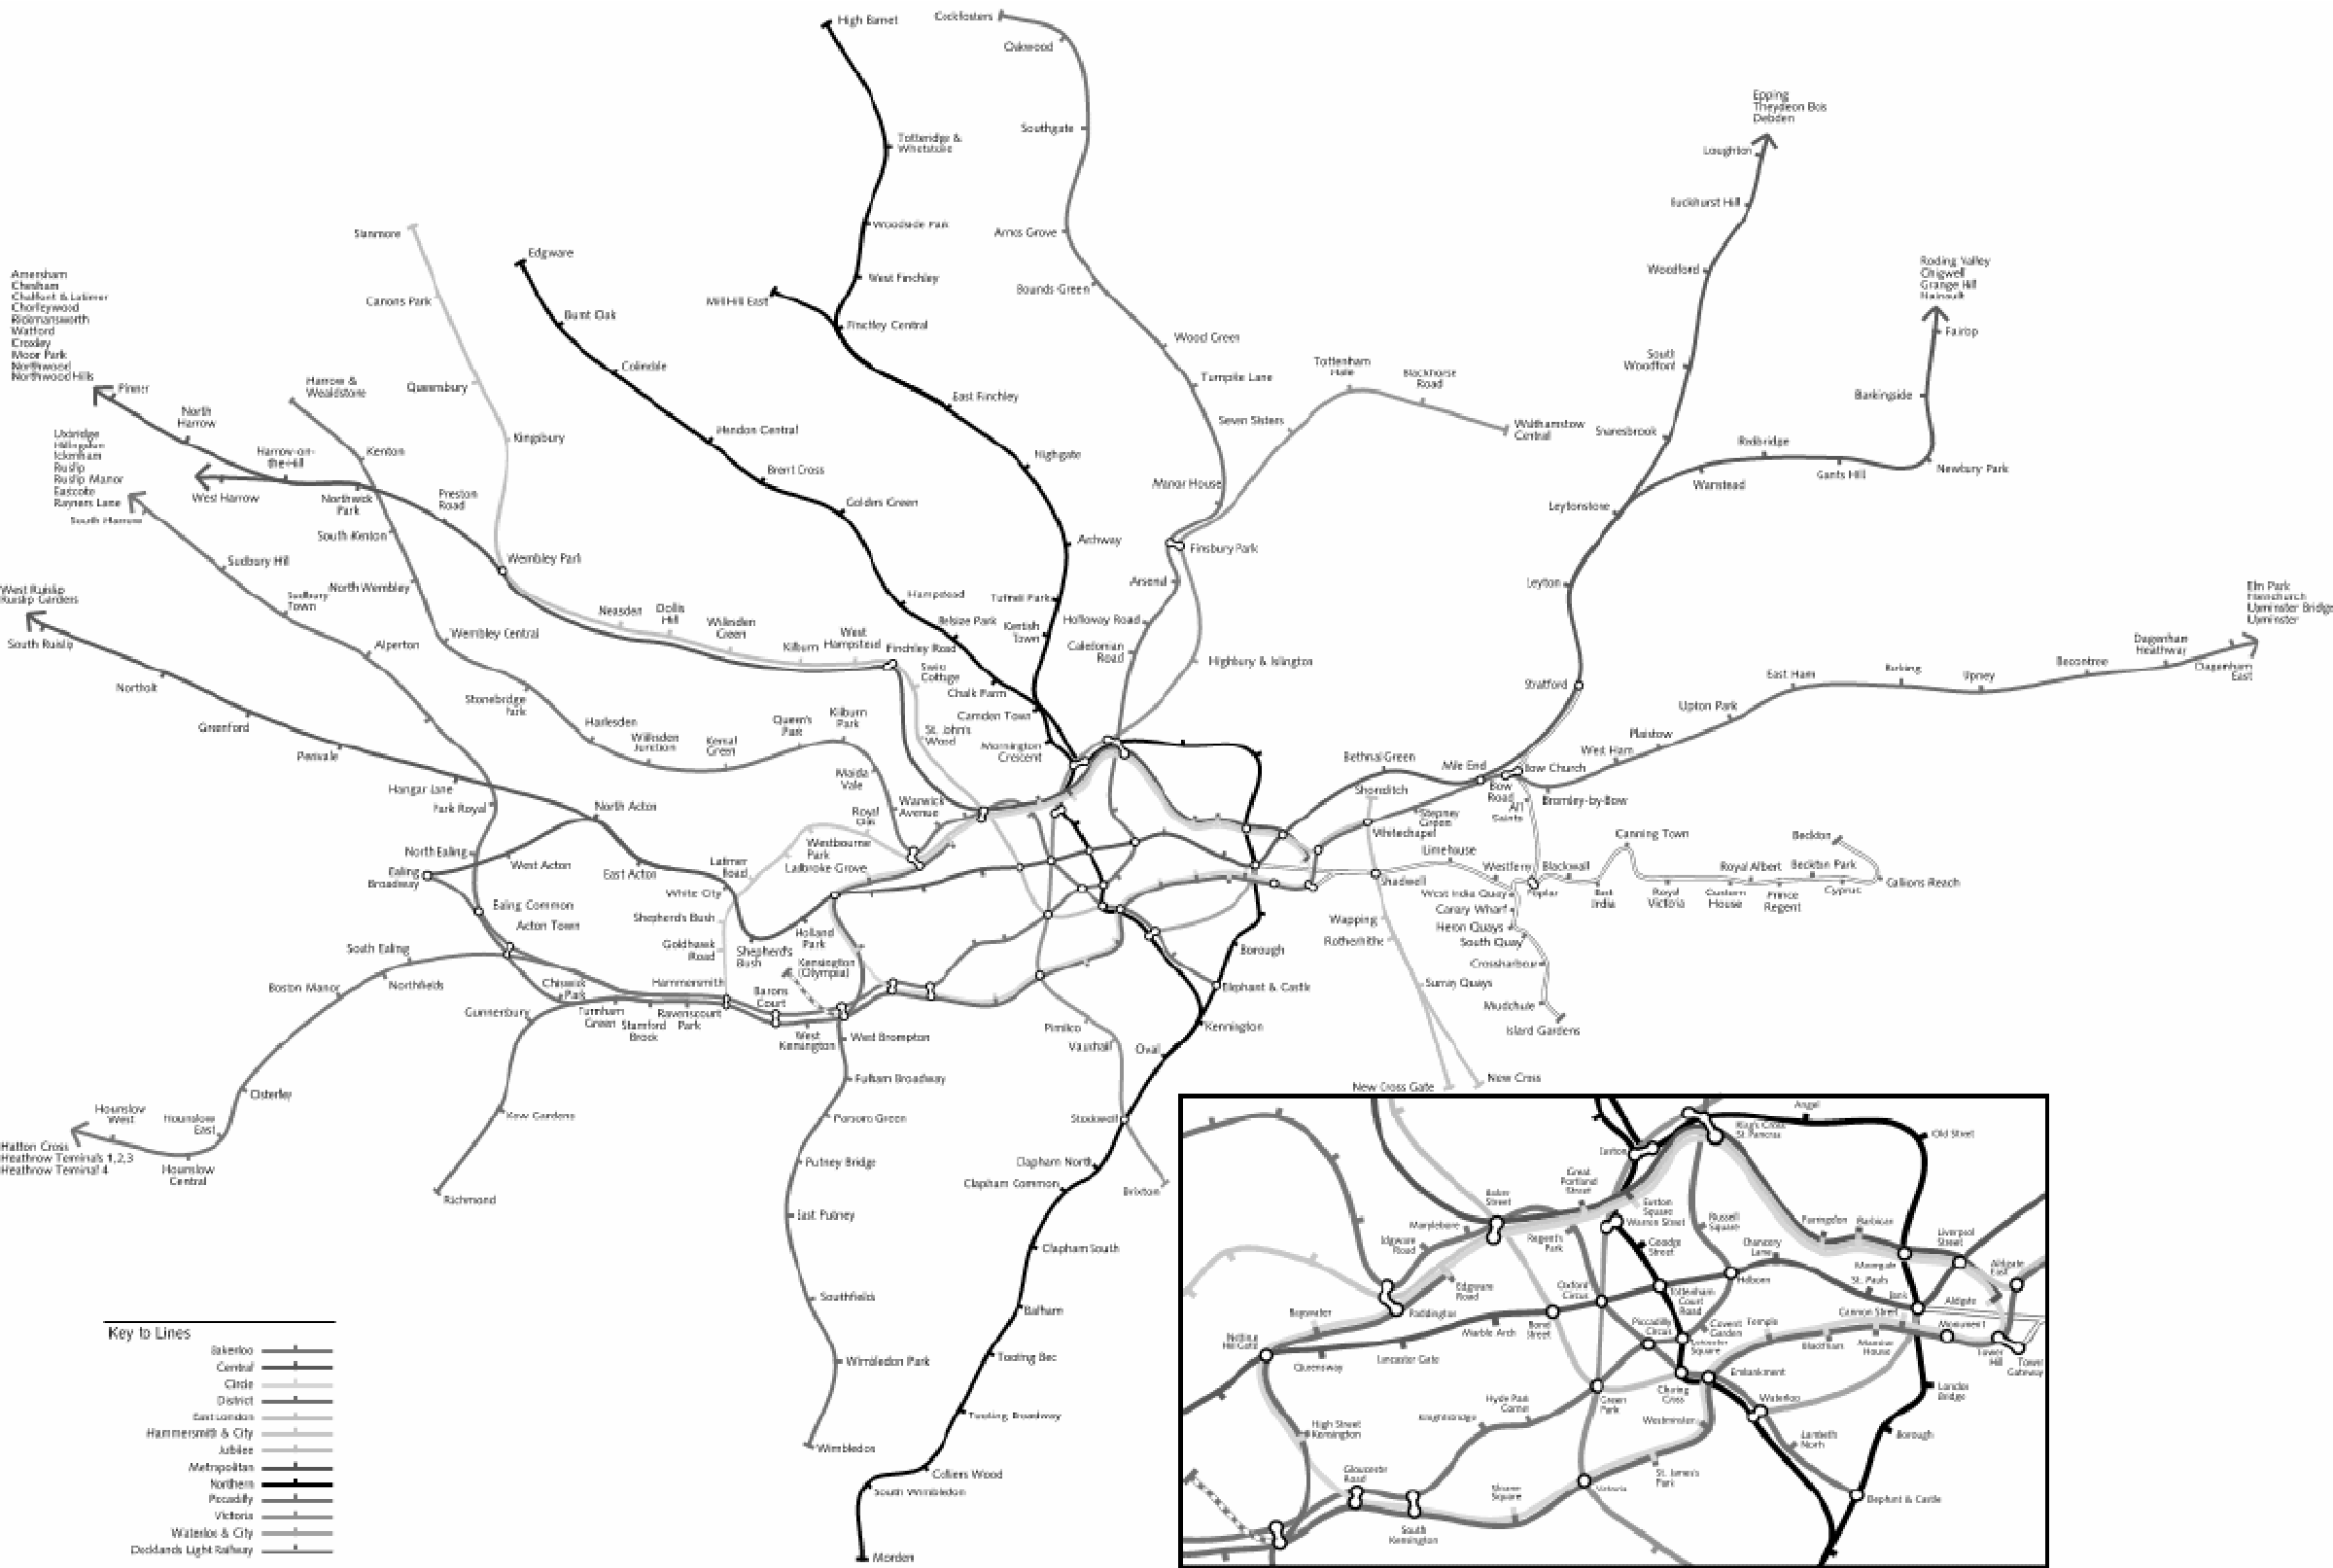
\includegraphics[width=5in]{geog}
\caption{\small The geographical representation of the London
                underground\label{train1}}
\end{figure}


\subsubsection{The Diagram}

Consider the following example based on that found in the excellent book 
{\em Using Z:
Specification, Refinement and Proof} by Jim Woodcock and Jim Davies:  \\

\noindent
Writing a specification at an appropriate level of abstraction is essential. 
A good example of this is provided by the various maps of the London 
Underground. When the first map was published in 1908, it was faithful to the 
geography of the lines: the shape of the track and distance between stations 
were faithfully recorded. However, the purpose of the map was to show 
travellers the order of stations on each line, and the various interchanges
between lines; the fidelity of the map made it difficult to extract this 
information. Figure~\ref{train1} shows the geographical representation of the 
London underground. \\

\noindent
The map was changed in 1933 to a more abstract representation which was 
rather nicely named \emph{The Diagram}. 
The draughtsman Harry Beck, who produced the imaginative yet stunningly 
simple design, based the map on the circuit diagrams he drew for his day 
job. All the detail concerning connectivity
was maintained, though the simplification meant that passengers could 
see at a glance the route to their destination. Abstraction from 
superfluous detail -- in this case the physical layout of the lines -- was 
the key to the usefulness of The Diagram. The Diagram 
can be seen in Figure~\ref{train2}. \\



\begin{figure}
\centering
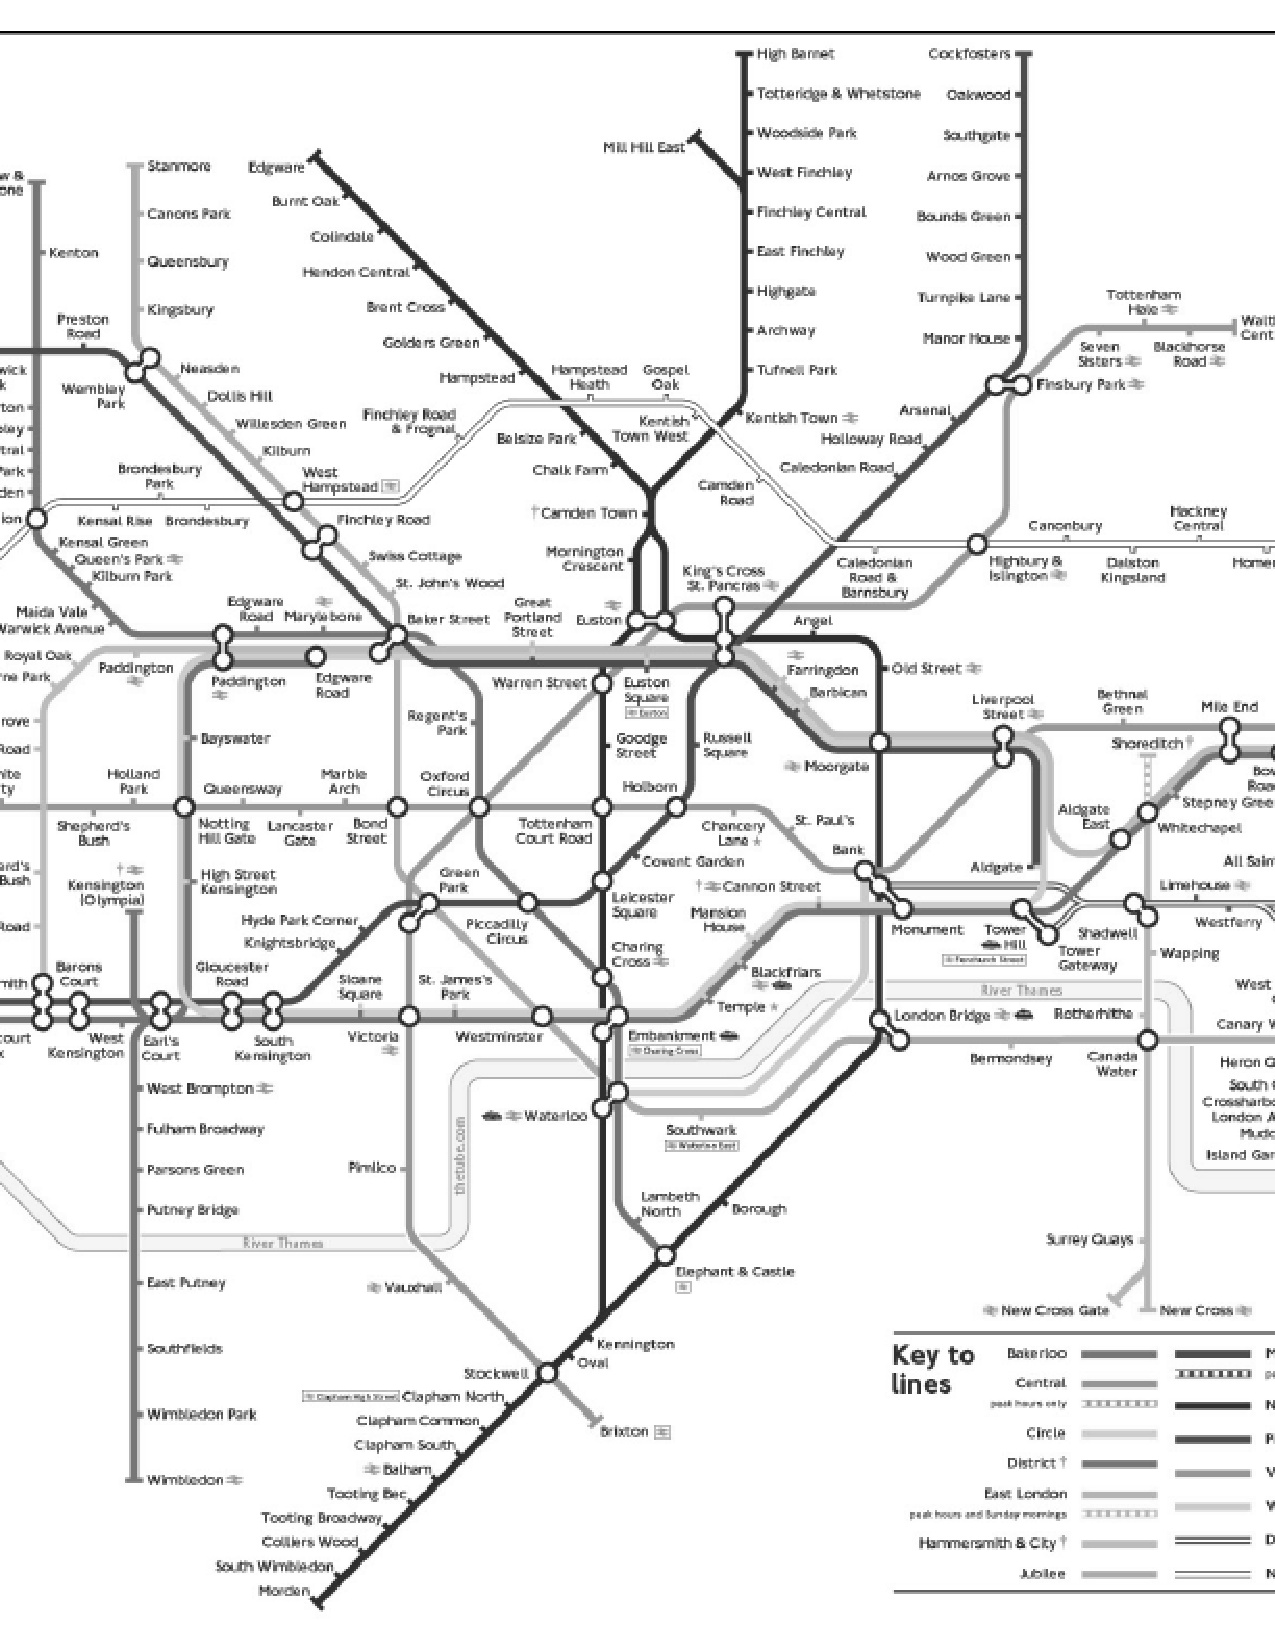
\includegraphics[width=5in]{tube_map}
  \caption{\small The Diagram, 1933; a more abstract description 
           \label{train2}}
\end{figure}

The Diagram was, and still is, a good specification of the London 
Underground. It is 

\begin{itemize}
\item
{\em Abstract}. Since it only records logical layout, not the physical 
reality in all its detail.

\item
{\em Concise}. Since it is printed on a single A5 piece of paper which is 
folded in such a way that it fits exactly into your pocket. 

\item
{\em Complete}. As every station on the London Underground network is 
represented.

\item
{\em Unambiguous}. Since the meaning of the symbols used is explained, and
the Diagram is represented in simple geometric terms. 

\item
{\em Maintainable}. Since it has been successfully maintained over the last
60 years, reflecting the changes to the network as new stations and lines 
have been opened and others have been closed. 

\item
{\em Comprehensible}. It must be readily understood by the general public. 
This has been the case as it has been regarded fondly by its users since 
1933. 

\item
{\em Cost-effective}. Since it only cost five guineas to commission the
specification from the engineering draughtsman Harry Beck. 
\end{itemize}

The Diagram gives its users a good conceptual model. It embodies a specification
structure that enables users to make sense out of a rather complex implementation. 
To do this it uses abstract shapes, colours and compression. All lines
are reduced to ninety or forty-five degree angles and the central area, 
where there are more stations, is shown in greater detail than the outlying 
parts, as if The Diagram were viewed through a convex lens. \\

The Diagram is an excellent example of a specification. You may be 
interested to know that it was first rejected by the Publicity Department of 
the London Underground, as the abstract notation was thought to be too strange
and incomprehensible for the ordinary user of the Underground network. 

\subsubsection{Writing your own specifications} 

Of course not all specifications can be dealt with in a nice pictorial form
such as The Diagram. Most specifications in fact use {\em Natural Language} and/or
some form of {\em Mathematics} or {\em Logic}. \\

Natural Language is perhaps the easiest way to communicate ideas, as most of 
us understand one language or another, English or Spanish for example. If you are to 
write specifications in a natural language then you must make sure that the
specification is unambiguous. The specification for a shampoo bottling firm
was unclear.

\begin{quote}
Line 10: Assign to the first variable the result of -- If the first bottle is
ready and there is some shampoo in the machine or the green light is on
then ...
\end{quote}

\noindent
We cannot be sure whether the `or' goes with the `shampoo
in the machine' part of the sentence, or with the 
`If the first bottle is ready and there is some shampoo in the machine' part 
of the sentence. \\

\noindent
We might make more sense of the definition by adding some mathematical notation
(brackets in this case),

\begin{quote}
Line 10: Assign to the first variable the result of -- (If the first bottle is
ready and there is some shampoo in the machine) or (the green light is on)
then ...
\end{quote}

\noindent
or by employing some logic

\begin{quote}
A = First bottle is ready \\
B = Shampoo is in the machine \\
C = Green light is on \\ 

Line 10: Assign to the first variable the result of -- ((A $\land$ B) $\lor$ C)
\end{quote}

\noindent
This final example uses some {\em Propositional logic}; three propositions are
defined (A, B and C) and they are combined using the logical 
AND ($\land$) and OR ($\lor$)
operators. The advantage that we see here is that the closer we move towards 
maths (or logic) the less chance there is of introducing any ambiguities. 

\subsection{Building computer programs}

Building a computer program is the task traditionally described
as {\em programming}. \\

\noindent
Despite many misconceptions, programming is not about sitting at a
desk full of cans of red bull and bashing out some obscure lines of text
which resemble the programmer's thoughts on a particular problem. Programming
is an exact and detailed science which involves translating {\em abstract} 
specifications
into more {\em concrete} implementations. The concrete implementation
is traditionally known as program {\em code}. 

\subsubsection{Abstract and concrete}

So what exactly is all this talk about {\em concrete} and {\em abstract}?\\

\noindent
You have seen already, in the description of a specification, that when we 
describe a problem which we may want to computerise, we should choose 
carefully the level of detail at which the problem is described. 
In writing a specification 
we must not get drawn in to any nitty-gritty points which are not
wholly in the domain of the problem itself. But why do we make such a
fuss about this, and does it really matter?\\

\noindent
Well, yes it does. When we program it is desirable to have as much freedom as 
possible: the freedom to choose a suitable programming language; choose 
our own structure and individual style; and maybe reuse bits of programs, 
to save time or money for example.  \\

\begin{figure}
\centering
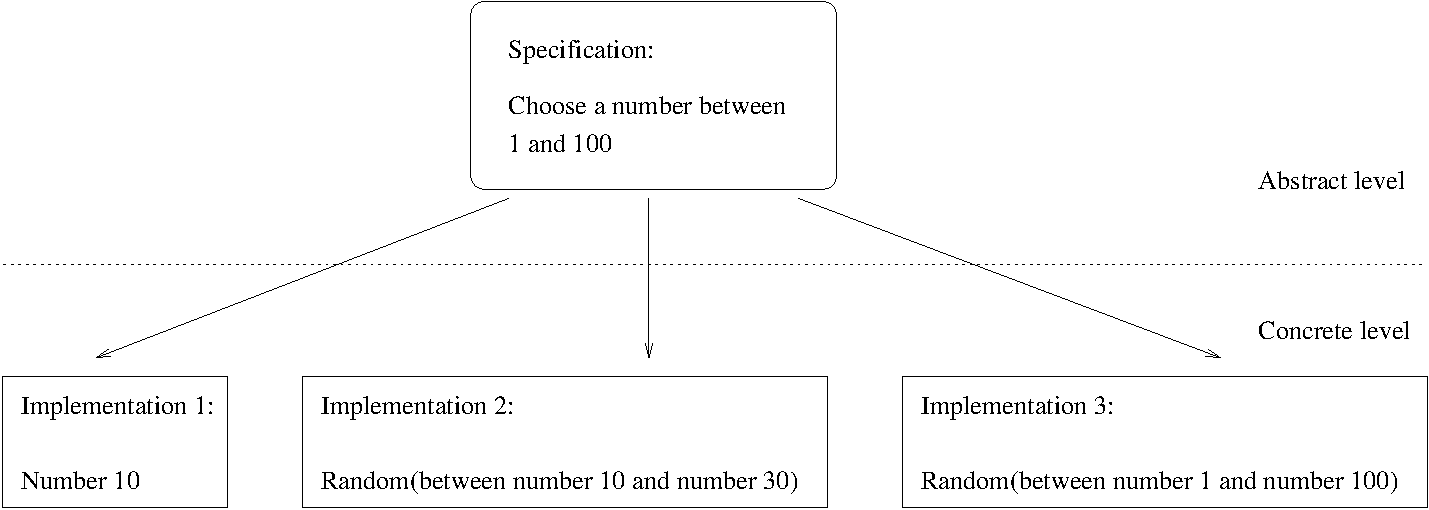
\includegraphics[width=5in]{abstract.pdf}
  \caption{\small Example of abstract- and concrete-level design 
           \label{specimp}}
\end{figure}

\noindent
In fact, it is possible to have many different programs 
which implement the same specification. Consider Figure~\ref{specimp} for example.
Here we have a specification which states, ``Choose a number between 1 and 
100''. There are three implementations of this specification in the figure: 

\begin{itemize}

\item
The first program simply produces the number 10. This, you may think, does
not meet the specification given, but think about it carefully. The 
specification says choose a number between 1 and 100, and the program does,
it chooses the number 10. It chooses the number 10 each time the
program is run of course, which 
is probably not what the person who wrote the specification wanted to happen.
But the specification does not say that the number chosen should be different
each time the program is run, so effectively the program is a perfectly 
good implementation of the specification. 

\item
The second program produces a random number between 10 and 30. This also 
meets the specification as the program certainly does choose a number 
between 1 and 100. Again, this is probably not what the person who wrote
the specification intended. 

\item
The third program is probably what you would have expected. It randomly chooses
a number 
between 1 and 100. This also meets the specification and had the 
specification been written more carefully, stating, ``...a different number
in this range should be chosen with equal chance each time the program is 
run...'', then this would be the only valid implementation of the 
specification written above.

\end{itemize}

\noindent
This may seem a little confusing. Why is it useful to have a number of 
possible computer programs which implement a single abstract specification?
The point is
that it may not matter to the customer exactly what the program does,  
provided that it is within the bounds of the specification. Therefore, the 
programmer has flexibility when producing a program, and the customer
receives a program which meets their requirements. Everyone wins. \\

\noindent
Abstract specifications are useful as they allow customers who might
be ordering a computer system to write a collection of unambiguous
requirements. They may pass this specification to a number of different
programmers and receive a number of different programs
back. Although these programs may be different and may be written in a
number of different programming languages, on a number of different
machines, they will all act
exactly as the specification states. The specification therefore acts
as a {\em contract} between the customer and the programmer, and a
contract between the abstract description and the concrete
implementation. 


\subsubsection{Translation}

Programming is the business of taking an abstract-level specification
and translating it into a concrete-level piece of code, and, as we have already seen,  programmers may
do this translation in an assortment of different ways. \\

\noindent
The translation between an abstract-level specification and a concrete-level
design is actually called {\em refinement}. Each of the programs
in Figure~\ref{specimp} is a valid refinement of the specification. \\

\noindent
Just as it is important to carefully write a specification, it is also 
important to make sure that the program implementation is an accurate
coding of the description in the specification. \\

\noindent
Usually a specification will have a number of complicated clauses, and 
may also span a number of pages. Although the specification 
may be exact in its description, a programmer may make a mistake 
when reading it and consequently code something different. For this 
reason, some specification methods have complicated mathematical rules 
which translate a piece of the specification (usually written mathematically)
into the corresponding piece of program code. These rules are 
known as {\em refinement rules}. You will learn more about these if
you choose to do the software specification course later in your degree.
 

\subsection{Testing computer programs}

Testing a computer program is an extremely important business. There are many
examples which I can cite where software has failed due to inadequate testing.
 Rather than 
bore you with a complete chronology, consider the following example:\\

\noindent
The story of Ariane 5 is a good one.
In the thrust direction control unit, 
code was reused from Ariane 4.
In this code, horizontal speed was represented
by a 16-bit value.
But horizontal speed in Ariane 5 was greater,
and caused an overflow, which raised an exception.
The specification said (very foolishly) that
if an exception arose, the processor should be 
shut down and restarted.
Shutting the processor down caused the thrust
direction to jump suddenly sideways, which
broke the rocket in half.\\

\noindent
Of course not every example of software failure will end in a disaster 
quite as catastrophic as this. However, the consequences of your code failing 
may prove to have just as much of an impact on the results of a small company,
or on the grade assigned to your computing assignment, for example. \\

\noindent
Testing is defined as the detection of failure; failure is the 
departure of the behaviour of a program from its requirements. Unfortunately,
it is not possible to show the absence of failure by testing, as testing 
will only tell us whether a program fails in a particular scenario or not.
The purpose of testing is to eliminate as many problems in the code as 
possible. This  
increases the programmer's (and user's) confidence in the piece of code. As
the number of failures detected in a program becomes less, the more you will 
feel that the program exhibits the correct behaviour.      

\subsubsection{Methods of testing}

The experimental science of software testing has been the subject of research
for a number of years. Consequently, there are a number of testing methods
which are shown to be effective. We will see, and use, a few of these methods
in this course. 

\paragraph{Test of logical paths of program} One useful way to test a program is to check all the logical
paths. Consider this example:

\begin{verbatim}
   while (x < 10) {
       if (even(x)) {
           System.out.println("The number is even\n");
        } else {
           System.out.println("The number is odd\n");
           x = x + 1;
       }
   }
\end{verbatim}

\noindent
To test the logical paths of this short piece of code the user would need 
to design tests to cover at least three cases: The case when {\tt x} is 
greater than or equal to 10, in which case the while loop would not be
executed at all; the case when {\tt x} is less than 10 and is even, in which 
case you would expect {\tt The number is even} to be printed at least once, 
and finally the test when {\tt x} is less than 10 and is odd, in which case 
you would expect {\tt The number is odd} to be printed at least once. \\

\noindent
Forgetting one of these cases will mean that you have not tested part of the 
code; this may be the piece of code which blows up, or
wipes the hard disk, or .... Would you expect any of the logical paths
in the program to reveal an error in the above code?

\paragraph{Range of inputs} Another way to test the example program would have been to test the range of 
inputs. If we can be sure that the program produces the right output for
each valid (and even invalid) input, then we can be a bit more sure that it
does what we expect. We may for example have tested the program with a 
negative value, a positive value and the value 0. \\

\noindent
Boundary cases are also important. You may want to check that the computer
deals correctly with the highest possible number and the lowest possible 
number. Finally, you may want to put some spurious values into the program --
what happens when you type in a character for example, or if you just press 
the enter key, or if you just sit on the keyboard?!\\

\noindent
Of course you have to select your range of inputs carefully. Selecting the 
numbers {\tt 137645813451875},  
{\tt 0.14643528745}, {\tt -23} and {\tt 19}, say, 
would not have found the infinite loop in the program.

\paragraph{Systematic tests} It is all very well to test the logical paths of the program and
the ranges of input, but it is sometimes the sequence of operations in
a program which causes it to break. For example, the `landing-gear down' and
`increase throttle' routines may both work exceptionally well by themselves, 
but putting the landing-gear down and then increasing the throttle may cause
the plane to head towards the ground at a rapid speed. This is probably not
what you want.  \\

\noindent
It may be worth testing a sequence of operations in your program, testing
all the permutations of the routines {\em a}, {\em b} and {\em c} for example,
to make sure that one does not exhibit any unexpected behaviour. 

\paragraph{Random tests} Random testing is a perfectly legitimate activity, but do not expect it to 
consistently come up with all the errors which may be detected by a logical or
systematic approach. \\

A true random test of a program is actually quite difficult to 
achieve. It would probably require a random number generator to 
choose between the routines in the program which were to be  
tested. A random test would also require a similar random 
selection activity to choose random input data to the program;
of course the amount of data itself must also be randomly chosen.
So be careful when you use the term `random testing'.
 
\paragraph{Intuitive tests} The process that people often think of as random testing is actually called {\it intuitive testing}. \\

After you have spent some time programming you may become aware of common
errors which appear in programs. A program which stores and deletes a 
collection of names will often be fooled if the first thing you ask it to 
do is to delete. Programs which accept characters as input will often break 
if you feed in a control character (which is a special character that cannot be printed
to screen).

Choosing cases like this to test your program is not a random 
activity -- you are usually selecting the tests based on your 
intuition as a programmer. So when you run a program for the 
first time and select a number of seemingly random operations, 
you will probably find yourself going through a number of cases
which you expect to work, followed by one or two cases in which 
you think the program may break. 

These tests usually require a bit of 
thought, but you can come up with some interesting results quite quickly. 
 

\paragraph{Test application} A {\em test application} is a piece of software which will run alongside the program to be tested. The test application may 
generate test data, supply tests, and record and calibrate the 
results as the testing takes place. Test applications are useful as they automate 
the testing process, removing any possibility of human error.
They also allow a large number of tests to be carried out 
automatically; you may for example run the test application over night, checking the 
results the following morning. \\

Test rigs also allow large systems to be tested with relative ease. Programmers
of large systems, those used by banks for example, often use test rigs 
when they are modifying the system. This means that the results before and after 
the modification can be compared to make sure that the system is still 
operating correctly. \\

One thing which is slightly ironic about test rigs is that they
themselves need testing, perhaps with test rigs, which themselves... \\

You might try some of these test methods later in the course. \\

The method of testing you use will often be dictated by a number of factors. 
You may not have time to carry out a logical or systematic test and an
intuitive test will have to do; it may be essential that you identify as many errors as 
possible, in which case random and range testing might not be good enough. It 
is up to you as a programmer to weigh up these factors to determine which 
method is appropriate given the situation. 
 

\clearpage
\section{Introduction to Java}

This chapter should serve as a Java reference throughout this course (and perhaps the CS126 course later this academic year). In this chapter the basic building blocks of Java programs will be outlined, with some short examples interspersed. If you have a question related to your coursework or exercise sheets, you should consult this chapter before asking for help from your seminar tutor.

Before we start discussing the ins and outs of Java, it's good to have a basic template in which to write all your code. Everything in Java is contained within a ``class'' (something that will be discussed fully later) and when a program is executed, as you will have done in Chapter 2, the Java environment looks for a particular method for an entry point to your code. For this quick introduction, you should create a file with the .java extension, and you should create a class in this file with a {\tt main} method. The \emph{main} method you write should have a specific function signature, where it should be declared {\tt public}, {\tt static} and {\tt void}, and it should have a single parameter that is an array of String objects. Specifically, your initial class declaration should look something like this,

\begin{verbatim}
public class MyClass {
public static void main(String[] args) {
...
}
}
\end{verbatim} 

After writing some logic in your main function, you can compile and execute the program as before.

\subsection{Variables}

In Java, we can use variables to store data, such that it can be reused or changed. Variable must be declared prior to their use and are given a symbolic name, and a \emph{type}. In this course you will use three forms of variables: \emph{primitive} variables, \emph{object} variables and \emph{arrays}.

\subsubsection*{Primitives}

\noindent
Java contains 8 primitive types that are the building blocks of all other types in Java. There are four \emph{integer} types, two {real} types, a character type and a boolean type. Specifically the primitive Java types are:

\begin{description}[style=multiline,leftmargin=2cm,font=\normalfont]
	\item[\tt byte] 8-bit integer type that can represent values between $-2^7$ and $2^7-1$. 
	\item[\tt short] 16-bit integer type that can represent values between $-2^{15}$ and $2^{15}-1$.
	\item[\tt int] 32-bit integer type that can represent values between $-2^{31}$ and $2^{31}-1$.
	\item[\tt long] 64-bit integer type that can represent values between $-2^{63}$ and $2^{63}-1$.
	\item[\tt float] 32-bit floating point type that can store approximately 6 digits of precision.
	\item[\tt double] 64-bit floating point type that can store approximately 15 digits of precision.
	\item[\tt char] 16-bit type that can represent any character in the UTF-16 character set.
	\item[\tt boolean] a type that can represent either {\tt true} or {\tt false}.
\end{description}

After deciding on an appropriate type, a variable needs a name, and possibly an initial value. The variable name can be any string of characters and number but cannot start with a number. Furthermore, variables can contain the underscore character ({\tt \_}) and a dollar sign ({\tt \$}), though its generally advised to not use dollar, and to not start a variable name with an underscore. Some names are also reserved; for example, a variable called {\tt int} would be incredibly confusing to the Java compiler, as well as a programmer.\\

Finally, a variable must be given a value before being used in subsequent statements. Variables are assigned using the \emph{assignment operator}, {\tt =}. Unlike in the world of mathematics, in most programming languages the value on the right, is assigned to the variable named on the left. For example $(1 + 2) \times 3 = x$ would be written in Java as: \\

\indent
{\tt int x = (1 + 2) * 3;}\\

\noindent
{\bf Exercise}\\

\noindent
Think about what each type above might be used for, e.g., the worlds population would require a {\tt long}, as it exceeds the range of an {\tt int}.\\

\noindent
The radius of the earth is approximately 6,371 km; the population is approximately 7,046,000,000 people. Try writing some Java statements to calculate the population density of the earth.

\begin{verbatim}
long population = 7046000000;
int earthRadius = 6371000;
double pi = Math.PI;
double surfaceArea = ...
\end{verbatim}

\subsubsection*{Objects}

There will be a more in-depth discussion of objects later in this guide, but one object variable you will come across is the String type. Object variable types usually start with a capital letter and are built from primitive variables. For instance, the String type stores all its data in arrays of {\tt char} types. Interaction with object types is usually done using the methods contained within the class. For example,

\begin{verbatim}
String s = "THIS IS A STRING";
System.out.println(s.toLowerCase());
System.out.println("The string is " + s.length() + " characters long");
\end{verbatim}

\noindent
The Java documentation is a great source to find what operations are valid on all of Java's in-built object types. Later in the course you will be designing and using your own object types.\\

\noindent
{\bf Exercise}\\

\noindent
Find the Javadoc documentation for the String class using google and find out how to find which character is at position $n$.

\subsubsection*{Arrays}

Finally, Java contains a special type for storing collections of similar objects. Arrays are declared in the same way as previous variable types but square brackets are used to indicate that there will be a collection of these objects. Further, arrays need to be given a length and from this point accessing individual items requires an index value. For example,

\begin{verbatim}
int myArray[] = new int[3];
myArray[0] = 3;
myArray[1] = 2;
myArray[2] = 3;
\end{verbatim}

\noindent
The {\tt new} keyword is used to initialise both object types and array types, and with arrays, requires a predefined size. Arrays in nearly all programming language begin at 0 and therefore the last item can be found at the location $n-1$, where $n$ is the length. In Java, the length of an array can be determined by checking the {\tt length} field of the array, e.g., {\tt myArray.length}.

\subsubsection*{Variable scope}

The final thing to say about variables right now is that they are very temporal creatures. They exist for a very limited amount of time, determined by their \emph{scope}. Specifically, from the point at which a variable is declared, it only exists within its enclosing braces. Variables declared outside of methods are called ``instance variables'' or ``class variables''. The difference between these two things will be discussed in lectures, but these variables maintain their values between different functions. Consider the following,

\begin{verbatim}
public class MyClass {
int instanceVar = 3;

public static void main(String[] args) {
int functionVar = 4;
}

public int myMethod() {
int functionVar = 5;
}
}
\end{verbatim}

\noindent
The variable {\tt instanceVar} exists throughout the whole class with the same value everywhere; a change to its value in {\tt myMethod}, would be reflected within all other methods. The two instances of {\tt functionVar} on the other hand only have scope from the point at which they are declared until the closing brace. Their values are independent and changing the value in {\tt myMethod} will not affect the other variable declared in the {\tt main} method. Variable scope will be covered more thoroughly in lectures; but the take away message is that variables have limited scope and cannot be accessed everywhere. Additionally, two variables with the same name may be allowed to coexist, providing their scopes do not overlap.

\subsection{Conditional statements}

Java programs are executed in-order, that is to say that when a Java application is executed, each line of code is executed in turn starting with the first statement in the {\tt main} method. There are often occasions where we do not want each line to be executed, for instance if we ask the user for two numbers and want to perform a division with them, if one of them is zero it is likely we do not want to perform a division by zero. To control the flow of Java applications, we use conditional statements.

\paragraph{If-statements} An if-statement is the simplest and most common conditional statement in Java and simply uses a condition that evaluates to true or false and executes code accordingly. To make an application execute one statement or another, an else statement can be attached to the end of the if-statement. Furthermore, you can join an if and an else statement to encode three possible choices. The basic format of an if-statement is:

\begin{verbatim}
if (condition) {
...
} else {
...
}
\end{verbatim}

\noindent
For example,

\begin{verbatim}
if (a < 0) {
System.out.println("a is less than zero!");
} else if (a == 0) {
System.out.println("a is equal to zero!");
} else {
System.out.println("a is more than zero!");
}
\end{verbatim}

\noindent
Conditions can also be chained using boolean algebra, where {\tt \&\&} indicates a logical-AND, and {\tt ||} indicates a logical-OR. Boolean conditions can be ``lazy'' or ``strict'', where a single {\tt \&} or {\tt |} character indicates strict evaluation and two characters indicate lazy evaluation. The distinction between these will be covered in lectures. When using complicated conditions in if-statements, be sure to bracket carefully to ensure clarity. For example,

\begin{verbatim}
if ((a == 0) && (b == 0)) {
System.out.println("Both a and b are 0!");
}
\end{verbatim}

\paragraph{Switch-statement}

The {\tt switch} statement is similar to an if statement evaluating the value of a specific variable to a specific value. However, the switch statement can behave in a more complicated way by allowing code to `drop through' many conditions. The basic format of a switch statement is:

\begin{verbatim}
switch (variable) {
case 1: ...
break;
case 2: ...
...
default: ...
}
\end{verbatim}

\noindent
With a statement of this kind, Java will look at the value of the variable, check if there is a specific case statement for its value, and begin executing instructions from this point onwards. If Java encounters a {\tt break} statement, it will skip to the end of the switch statement and continue with the application. Because a break statement is required to stop code from executing, if there is no break between two cases, Java may execute the code for both cases even through only the first matched the variable. If no cases are matched, the {\tt default} case will be executed, unless it is absent.\\

\noindent
{\bf Exercise}\\

\noindent
Try converting the following if statement into a switch statement, using the fact that a switch statement will drop through many conditions when there is no break statement:

\begin{verbatim}
if ((a == 1) || (a == 2) {
System.out.println("a is one or two");
} else if (a == 3) {
System.out.println("a is three");
} else {
System.out.println("a is neither one, two or three");
}
\end{verbatim}

\noindent
Now try converting the following switch statement into an if statement:

\begin{verbatim}
switch (a) {
case 5:
case 7:
case 8: System.out.println("a is five, seven or eight");
break;
case 1: System.out.println("a is one");
case 2: System.out.println("a is two");
break;
default: System.out.println("a is something else");
}
\end{verbatim}

\subsection{Iteration statements}

While coding Java applications you may find that you end up repeating yourself. Repeated code can be encapsulated into an iteration statement to make Java execute the same code multiple times. Consider,

\begin{verbatim}
int a = 1;
System.out.println("a is: " + a);
a = a + 1;
System.out.println("a is: " + a);
a = a + 1;
System.out.println("a is: " + a);
a = a + 1;
\end{verbatim}

\noindent
Using an iteration statement this code can be condensed to many fewer lines, and the repeated action can be increased without having to add additional lines of code. As with almost all coding, this can be achieved in multiple ways. In this course we will deal with while loops and for loops, as well as some variants on these.

\subsubsection*{While-loops}

A while loop can be thought of as a repeating if statement, where the body of the if will be continually executed until the condition is no longer met. Specifically they are coded like so:

\begin{verbatim}
while (condition) {
...
}
\end{verbatim}

\noindent
To encode the previous code into a while loop we may do something like the following,

\begin{verbatim}
int a = 1;
while (a < 4) {
System.out.println("a is: " + a);
a = a + 1;
}
\end{verbatim}

\noindent
When using while loops, you should be careful to ensure that the condition changes, otherwise an infinite loop may exist in which the program will continually execute the middle block without ever finishing. Consider what might happen if you removed the statement {\tt a = a + 1} in the example above. The code would print {\tt a is: 1} until the end of time, and this was probably not what was required.\\

\noindent
There are some cases where you would like the condition to be evaluated \emph{after} the body has been executed, ensuring that the body will be executed at least once. For this we can use a do-while loop like so:

\begin{verbatim}
do {
...
} while (condition);
\end{verbatim}

\noindent
A good reason to use a statement like this would be if you wanted to assign a value to a variable and change it only under certain conditions. You may find this form of loop beneficial for the robot-maze coursework. Consider the following example,

\begin{verbatim}
double a;
do {
a = Math.random();
} while (a < 0.5);
\end{verbatim}

\noindent
This would pick a random number for {\tt a} and then continually pick new a one until {\tt a} is greater than or equal to 0.5.

\subsubsection*{For-loops}

Sometimes you may want a loop to iterate a variable over a very specific range of numbers, or for a specific number of times. While this is possible with a while-loop, for these situations we often use a for loop. A for loop is written using three components: an initial condition, an terminating condition and an iterative operation. For example,

\begin{verbatim}
for (initial condition; termination condition; iteration operation) {
...
}
\end{verbatim}

\noindent
Rewriting the while loop at the beginning of this section as a for loop would make for even more concise code, as the variable declaration and incrementation operation are included as part of the loop.

\begin{verbatim}
for (int a = 1; a < 4; a = a + 1) {
System.out.println("a is: " + a);
}
\end{verbatim}

\noindent
{\bf Exercises} \\

\noindent
Rewrite the following for-loop as a while-loop:

\begin{verbatim}
for (int a = 10; i > 0; i = i-2) {
System.out.println("i is: " + i);
}
\end{verbatim}

\noindent
Given the following code, copy the characters out of the String {\tt s}, in to the {\tt char} array {\tt c}. Use the Javadoc for String to find out how to retrieve individual letters from {\tt s}. Try using both a while and a for-loop.

\begin{verbatim}
String s = "This is a string";
char c[] = new char[s.length()];
...
\end{verbatim}

\subsection{Input and output}

Computer systems normally have three ``streams'' that can perform input and output (I/O) to and from the users console. Two of these streams are for writing data out, and they are the output stream and the error stream, and the final stream is the input stream. In Java these can be found under the {\tt System} class as {\tt System.out}, {\tt System.err} and {\tt System.in}. We've already been writing out to the \emph{output} stream using the {\tt println()} method; you can write out on the error stream in the same way, but instead of {\tt System.out}, we use {\tt System.err.println("...");}. To find more things you can do with {\tt System.out} and {\tt System.err}, you can look up the {\tt PrintStream} Java documentation. You should find a method called {\tt print()} that works like {\tt println()}, but doesn't put a line-break at the end; this can be used to build strings on the output, instead of concatenating things beforehand. For example:

\begin{verbatim}
String s = "This"
s = s + " is a string";
System.out.println(s);

System.out.print("This");
System.out.print(" is a string");
System.out.println();
\end{verbatim}

\noindent
Both bits of code will produce the same output, but the second can be done over the course of an exercise without subsequent additions being placed on new lines.\\

\noindent
For input streams, data has to be read either byte-by-byte or by using another class to do this for us. Luckily, Java provides the {\tt Scanner} class exactly for this purpose. First, a Scanner object is created and assigned to a variable, and then its methods can be called to retrieve user input. For example:

\begin{verbatim}
Scanner sc = new Scanner(System.in);
long aLong = sc.nextLong();
double aDouble = sc.nextDouble();
\end{verbatim}

\noindent
This will first read in a value as a long and then read a value as a double. Explore the {\tt Scanner} documentation to find more interesting uses of Scanner before proceeding to the following exercise.\\

\noindent
{\bf Exercise}\\

\noindent
Using your knowledge of loops and the documentation for Scanner, use the {\tt nextDouble()} and {\tt hasNextDouble()} to read in numbers until something that is not a number is encountered and then output the total of the doubles encountered. Your output should look something like this:

\begin{verbatim}
Enter double: 4.5
Enter double: 5.2
Enter double: blah
The total of the doubles entered was: 9.7
\end{verbatim}

\subsection{Methods}

You've already been using methods throughout this chapter. You differentiate methods from variables by the use of the following brackets, {\tt ()}. Breaking down problems into subproblems, you may find that some operations are repeated; extracting these behaviours into methods allows sensible code reuse, decreasing the amount of coding required and facilitating future extensions. In Java, the terms method, function and subroutine are used interchangeably, though outside of the Java-world, their definitions vary subtly. All methods in Java have a name, a list of parameters and a return type. There is a special type that can be used when no return value is required, we call this type {\tt void}. You've already seen a {\tt void} function in Java, as the {\tt main} method does not return any value to the computer. Further to this, methods also require an \emph{access modifier} ({\tt public}, {\tt private} or {\tt protected}), which we will cover in the next section. The basic format of all function declarations follows the following form:

\begin{verbatim}
[access] [type] methodName([type] varName, [type] varName, ...) {
...
}
\end{verbatim}

\noindent
Where {\tt access} is either {\tt public}, {\tt private}, or {\tt protected}, and {\tt type} is a variable type. Thus, a basic add function that takes two inputs and returns the sum of the two may look something like:

\begin{verbatim}
public int add(int a, int b) {
return a + b;
}
\end{verbatim}


\noindent
Here the method is made public and will return an integer value. There are two inputs to the method, called {\tt a} and {\tt b}, and they are also integer values. Java requires that methods which have a non-void return type, explicitly return a value using the {\tt return} keyword. You would call this method and provide two values (or variables) to the method with a function call like so:

\begin{verbatim}
int c = add(3, 4);
\end{verbatim}

\noindent
As state previously, some methods may not need to return a value and can be declared {\tt void}. For example, if a method writes a String to the screen, it may not need to return a value to the program:

\begin{verbatim}
public void printError(String errorstring, int errornumber) {
System.err.println("Error number " + errornumber +
": " + errorstring);
}
\end{verbatim}

\noindent
{\bf Exercise}\\

\noindent
Given the formula:
$$x = \displaystyle\frac{-b \pm \sqrt{b^2 - 4ac}}{2a}$$

\noindent
Write a function to calculate $x$. You may want to look up the Math java documentation to find methods for square root and powers. You may also require two functions, one to return the result with a positive determinant, one for the negative case. Unless you're feeling very brave, ignore the cases where there are complex roots.

\subsection{Object-oriented programming}

In Java, whether you've realised or not, (almost) everything is an object. You've been writing classes, which you can think of as a blueprint for an object. Specifically, an object is an instance of a class and is initialised with the {\tt new} keyword. Consider the Scanner class:

\begin{verbatim}
Scanner sc = new Scanner(System.in);
\end{verbatim}

\noindent
This is creating an object variable called {\tt sc}, and it is initialising it to be a new instantiation of the Scanner class. Furthermore, it is calling a special method that exists in the Scanner class called a \emph{constructor}. Constructor methods have the same name as the containing class, and have no return type. These methods are used to initialise instance variables (i.e. variables with scope across an entire instance of a class) and potentially call some set up functions. From this point on the object can be used much like the Scanner class is used, calling functions by using the instance variable name, a stop and the name of the function ending with bracketed parameters. Consider the following example:

\begin{verbatim}
public class MyClass1 {
public static void main(String[] args) {
MyClass2 mc = new MyClass2(4);
System.out.println(mc.getA());
}
}

class MyClass2 {
private int a;
public MyClass2(int a) {
this.a = a;
}

public int getA() {
return a;
}
}
\end{verbatim}

\noindent
This example contains two classes, {\tt MyClass1} and {\tt MyClass2}. The first class has a main method and is therefore where execution begins. It creates an object called {\tt mc}, and initialises it using the {\tt MyClass2} constructor method to set the instance variable {\tt a}. As {\tt a} is declared twice in the class, the {\tt this} keyword is used to differentiate between the instance variable {\tt a} and the method variable {\tt a}; {\tt this.a} refers to the instance variable, whereas {\tt a} refers to the parameter passed to the constructor method.\\

\noindent
After creating the object, the method {\tt getA()} is used to get the value of {\tt a} and return it such that it can be printed with the {\tt println()} function.

\subsubsection*{Access modifiers}

If you've been paying careful attention so far, you'll have noticed that words such as {\tt private} and {\tt public} have been dotted around before variable and method declarations. These are fundamental features of all object-oriented programming languages and allow us to make use of \emph{encapsulation}. When writing object oriented code, we generally follow the rule of {\bf private variables, public methods}. What this means is that our class variables must be private and can therefore only be changed by method in the class. Imagine a ATM system that is programmed like this:

\begin{verbatim}
public class BankAccount {
String name;
long accountNumber;
double balance;
...
public double withdrawFunds(double amount) {
if (balance > amount) {
balance = balance - amount;
return amount;
} else {
System.err.println("You do not have enough money!");
return 0;
}
}
}
\end{verbatim}

\noindent
Money is withdrawn from the machine using the {\tt withdrawFunds()} method, which can check the available balance beforehand and warn the user if a transaction is not allowed. In this example the instance variables are not given an access modifier and are therefore implicitly \emph{public} and can be changed by another class like so:

\begin{verbatim}
BankAccount b = new BankAccount("Bob", 1235323, 1000.0);
b.balance = b.balance - 1100.0;
\end{verbatim}

\noindent
Here, the balance variable has been manipulated directly and so no check has been made to see if the action is valid. If the variables are made \emph{private}, then we can only manipulate them using predefined methods that can perform additional operations. Therefore, it would be better to write this class like so:

\begin{verbatim}
public class BankAccount {
private String name;
private long accountNumber;
private double balance;
...
}
\end{verbatim}

\noindent
This is not to say that all your variables should be private and all your methods should be public. Infact, the safest way to program is to make all things private unless external access is required (i.e. you have another class that needs to perform a particular action).

\subsubsection*{Inheritance}

The final thing to say on object oriented programming in this quick-stop guide is on the subject of \emph{inheritance}. One of the most powerful facets of Java and other object oriented programming languages is that you can create classes that inherit properties and methods from other classes, allowing you to take advantage of existing code and allowing you to build an object hierarchy. This may seem strange but consider the furniture you have at home. Many of the items share some properties and functions but also require some different properties. Let's create a class for furniture.

\begin{verbatim}
public class Furniture {
private String material;
private double weight;
...
}
\end{verbatim}

\noindent
Now think about your dining room table and chairs. They're both forms of furniture, but they have different properties, thus we can {\tt extend} the Furniture class and inherit the methods and properties that all items of furniture share, and add our new functions and properties.

\begin{verbatim}
public class Chair extends Furniture {
private short numberOfLegs;
...
}

public class Table extends Furniture {
private short numberOfLegs;
private int length;
private int width;
...
}
\end{verbatim}

\noindent
We can even extend the extended classes, to create a specialisation for an office chair, or a stool, or an exam desk with an integrated chair!\\

\noindent
{\bf Exercise}\\

\noindent
Starting with a class for animals, try writing a series of classes for cats, dogs, spiders and flies. It may be beneficial to have intermediate classes such as a Mammals class. Don't worry too much about the implementation of the functions, just think about how properties are shared by all of the subclasses.

\subsection{Debugging Java}

The final section of this whistle-stop tour of Java is perhaps the most important of all. When you encounter problems with the code you have written, before approaching a seminar tutor, your friends or me, you should attempt to fix the problem yourself. Luckily, Java provides perhaps the best, most informative error messages of all compilers/programming languages. Consider the following code (with added line numbers!):

\begin{verbatim}
1: public class Test {
2:    public static void main(String[] args) {
3:        System.out.println(a);
4:    }
5: }
\end{verbatim}

\noindent
If we try to compile this code, we get an error message like so:

\begin{verbatim}
$ javac Test.java
Test.java:3: error: cannot find symbol
System.out.println(a);
^
symbol:   variable a
location: class Test
1 error
\end{verbatim}

\noindent
Here we see that the Java compiler has told us that the error is in Test.java and is on line 3. The error ``cannot find symbol'' means that a particular variable or method (which Java calls symbols) cannot be found. Furthermore, the compiler tells us which symbol it cannot find (variable {\tt a})!\\

\noindent
{\bf Exercise}\\

\noindent
Fix this error!\\

\noindent
The error you just encountered is called a \emph{syntactic} error, and occurs at compile time. There is an error in the syntax of the code and this cannot be understood by the Java compiler. Throughout this course you may also encounter \emph{semantic} errors. These are errors where the meaning of the code has been understood by the compiler, but the logic is incorrect. Consider the following:

\begin{verbatim}
1: public class Test {
2:    public static void main(String[] args) {
3:        int a[] = new int[2];
4:        a[2] = 3;
5:    }
6: }
\end{verbatim}

\noindent
The code above compiles without error, but when running the program we see that there is an \emph{exception} in the code. Again, Java does a good job telling us about the error:

\begin{verbatim}
$ javac Test.java
$ java Test
Exception in thread "main" java.lang.ArrayIndexOutOfBoundsException: 2
at Test.main(Test.java:4)
\end{verbatim}

\noindent
The error is in the {\tt main} function in Test.java and is on line 4. The exception that was generated was an ArrayIndexOutOfBoundsException (which you can look up in the Javadoc) and has occurred because we are trying to store a number in a location in the array that is out of bounds. If you remember, when we create an array of a particular size, the last index is $n-1$. Here we're trying to write something into array index 2 (which the error tells us), but the array only contains space for 2 integers, at index 0 and 1.\\

\noindent
{\bf Exercise}\\

\noindent
Try writing example applications to perform very simple tasks. While doing this, you will undoubtedly encounter errors and you should now be able to identify exactly where and what the errors are. Try to learn about as many error types as possible and how to fix them, this will benefit you greatly in the future.



\clearpage
\section{Introduction to the Robot Maze}

The coursework exercises for this year's CS118 module are based on a simulated ``Robot Maze'' environment.  A small robot has been designed to be able to navigate its way through mazes to find a target at some given location.  This task resembles those used in the classic learning 
experiments of the 1960s which included laboratory
mice (and cheese, mild electric shocks, mice of the opposite sex, etc).
The objective of the robot (or mouse as it was then) or, more generally, the \emph{agent} is to 
find the given target as rapidly and efficiently as
possible, learning the maze over several runs and so on.  

Building a real robot and a real maze requires a combination of efficient 
sensors and mechanics, sophisticated steering and speed control, clever 
maze exploration and navigation procedures and, no doubt, a good deal of
glue.  For the purpose of these exercises we focus
entirely on designing the maze exploration and navigation algorithms.
We make no attempt to model the physics of a moving wheeled (or legged!)
robot and concentrate solely on the part of the 
problem which can best be solved with software. 

\subsection{The Robot Maze environment}

The simulated Robot Maze environment has the following characteristics:

\begin{itemize}

\item The robot moves through a simple square-block maze of the type
  illustrated in \Cref{maze}.  The floor space of the maze is divided into squares of uniform size. Each square is either occupied by a wall or is empty.

\item The robot occupies exactly one non-wall square and moves in
  discrete steps, one square at a time, north, south, east, or west.
  The robot cannot move diagonally.  If the robot attempts to move
  outside the boundary of the maze or into squares occupied by walls it
  suffers a harmless collision (indicated by flashing red in the
  simulation) and stays in the same square.

\item The direction the robot moves in is determined by the direction it is facing (its heading, indicated by an arrow in the simulation).  The robot can change the direction it is facing by rotating on the spot. Each of these rotations are directed by the robot's control procedure -- a method called \javaIn{start} -- which is run at the start of a simulation. 

\item A simulation \emph{usually} starts with the robot at the top left-hand square of the maze and ends when either the robot reaches the target or the user loses patience and stops the robot (by pressing {\bf Reset} in the user interface). The target square is usually the bottom right-hand corner of the maze, but this along with the robot start position can be modified by the user. 

\end{itemize}

\begin{figure}
\centering
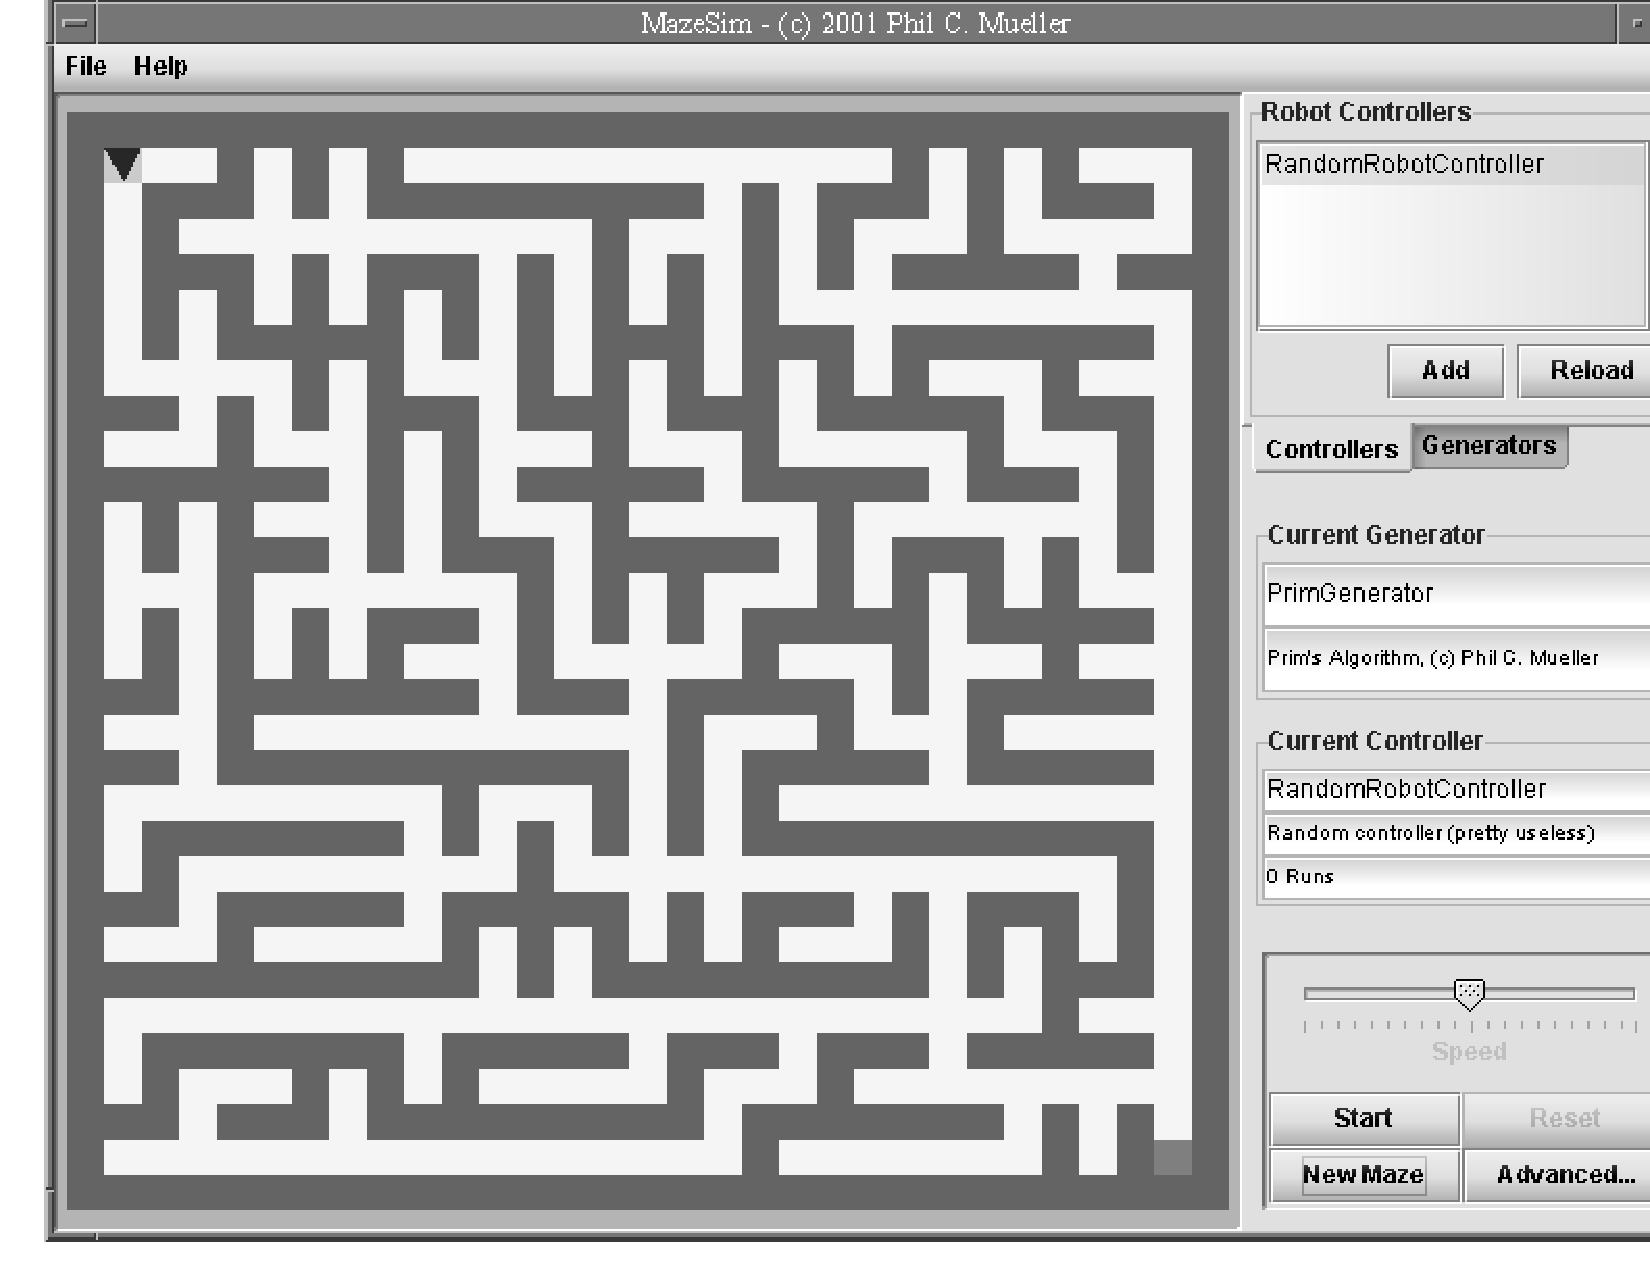
\includegraphics[width=10cm]{maze.pdf}
\caption{The Robot-maze environment\label{maze}}
\end{figure}

During its execution the robot's control program (which you are required to
write) has access to the following information:

\begin{itemize}

\item The direction the robot is currently facing;

\item The status of the squares ahead, behind, left and to the right of the robot. Squares are either walls, empty, or squares the robot has been at before (which are otherwise empty squares). The boundaries of the maze are treated as walls;

\item The {\it x} and {\it y} co-ordinates of the square the robot is currently occupying, and those of the target square;

\item How many attempts the robot has made at traversing the given maze.
\end{itemize}

\subsection{Programming robot control programs}

The simulated robot maze environment is written in Java. The programs which you are required to write for this module are also Java-based which means that you will be writing code which directly hooks into this robot maze environment. 

To allow this hook-up, there needs to be a common interface between the robot maze Java code and your own Java code. This interface is documented in the following sections. However, since you are only required to write control software for the maze environment and while every part of the maze software is accessible for you to use, the implementation of the maze environment itself is hidden from you. This is an example of abstraction. Everything you need to know to use the maze environment is documented in this guide.

The information listed below is important and you should make sure that you understand what it all means. If you are not clear on anything then you might like to talk about it with your peers first and then ask for clarification from the teaching team. Understanding \emph{program interfaces} like this is very important in software development, particularly if you are to use it to write your own program code.

\subsubsection{Specifying headings in the maze}

Four pre-defined constants are defined in the code for the robot maze program to specify directions in the maze. These are

\javaIn{IRobot.NORTH}, \javaIn{IRobot.EAST}, \javaIn{IRobot.SOUTH}, \javaIn{IRobot.WEST}

where the maze follows the usual mapping convention of having \javaIn{IRobot.NORTH} upwards and \javaIn{IRobot.EAST} to the right etc.

As the values are defined as part of a Java interface named \javaIn{IRobot}, the constants are prefixed with the name of the interface as shown above when they are used in the actual program code that you write. This might seem a bit quirky but you will 
soon get used to it. 

These elements of the interface are concretely represented as Java values of type \javaIn{int}. The values represented by these directional constants are chosen so that the following equalities hold:

\begin{center}
\begin{tabular}{rcl}
\javaIn{IRobot.NORTH+1} & \javaIn{==} & \javaIn{IRobot.EAST}	\\ 
\javaIn{IRobot.EAST+1} & \javaIn{==} & \javaIn{IRobot.SOUTH}	\\ 
\javaIn{IRobot.SOUTH+1} & \javaIn{==} & \javaIn{IRobot.WEST}	\\ 
\end{tabular}  
\end{center}

\taskLine 

\task{Note that \javaIn{IRobot.WEST+1 != IRobot.NORTH}. Could you find a way to represent the directions in Java so that this would be the case?}

\taskLine 

\subsubsection{Specifying directions relative to the robot heading}

Four pre-defined constants are defined in the code for the robot maze program to specify directions relative to the robot's current heading. These are:

\javaIn{IRobot.LEFT}, \javaIn{IRobot.RIGHT}, \javaIn{IRobot.AHEAD}, \javaIn{IRobot.BEHIND}

As with headings these are also of the type \javaIn{int}. The values represented by these directional constants are chosen so that the following equalities hold::

\begin{center}
	\begin{tabular}{rcl}
		\javaIn{IRobot.AHEAD+1} & \javaIn{==} & \javaIn{IRobot.RIGHT}	\\ 
		\javaIn{IRobot.RIGHT+1} & \javaIn{==} & \javaIn{IRobot.BEHIND}	\\ 
		\javaIn{IRobot.BEHIND+1} & \javaIn{==} & \javaIn{IRobot.LEFT}	\\ 
	\end{tabular}  
\end{center}

A fifth constant \javaIn{IRobot.CENTRE} is also defined, which can be useful as a ``do nothing'' value when communicating values between parts of complex control programs.

Do not be put off by the fact that these values have an \javaIn{int} type. As far as the control programmer (this is you) is concerned, all references to headings and directions are done using the constant \emph{name} (i.e. \javaIn{IRobot.RIGHT}, 
\javaIn{IRobot.NORTH}, etc.) and not the constant \emph{value} used to represent it. This is our first encounter with \emph{program abstraction}. 

\subsubsection{Sensing the squares around the robot}
\label{lookmethod}

The method \javaIn{robot.look(direction)} takes a value
specifying a direction relative to the robot (e.g. \javaIn{IRobot.AHEAD} or \javaIn{IRobot.LEFT}, etc.) and returns a value which indicates the state of the corresponding square neighbouring the robot. The possible states are:

\begin{tabular}{r|p{0.6\textwidth}} 
	\javaIn{IRobot.PASSAGE} &  An empty square that has not yet been visited on the current traversal of the maze. \\ \hline 
	\javaIn{IRobot.WALL} & An empty square that
	has already been visited during the current traversal of the maze. \\ \hline  
	\javaIn{IRobot.BEENBEFORE} & A wall or the edge of the maze \\
\end{tabular} 

\begin{figure}
\begin{subfigure}[t]{0.5\textwidth}
	\centering
	
\includegraphics[width=0.5\textwidth]{mousemove_new}
\end{subfigure} 
~
\begin{subfigure}[t]{0.5\textwidth}
	\centering
	\begin{tabular}{l l} 
		\textbf{Function call} & \textbf{Result} \\ \hline
		\javaIn{robot.look(IRobot.AHEAD)}  & \javaIn{IRobot.WALL} \\
		\javaIn{robot.look(IRobot.BEHIND)} & \javaIn{IRobot.BEENBEFORE} \\
		\javaIn{robot.look(IRobot.LEFT)}   & \javaIn{IRobot.WALL} \\
		\javaIn{robot.look(IRobot.RIGHT)}  & \javaIn{IRobot.PASSAGE} 
	\end{tabular}
\end{subfigure}

\caption{Example of sensing robot surroundings\label{sensing}}
\end{figure}

\Cref{sensing} shows a typical situation that might arise during a
traversal of the maze. The robot is located in the square with an arrow, facing in the direction of the arrow, with squares visited previously during the same run shaded in grey. The walls are in black. In this situation \javaIn{robot.look} would return the results shown in the table.

If the robot chooses to turn right and then move forward one square, then a call to the method \javaIn{robot.look(IRobot.AHEAD)} would return \javaIn{IRobot.PASSAGE}.

\subsubsection{Sensing and setting the robot's heading}

The method \javaIn{robot.getHeading()} returns the robot's current heading in the maze. That is either \javaIn{IRobot.NORTH}, \javaIn{IRobot.SOUTH}, \javaIn{IRobot.EAST}, or 
\javaIn{IRobot.WEST}. In the example in \Cref{sensing} a call to the method \javaIn{robot.getHeading()} would return the value \javaIn{IRobot.EAST}. There is a ``sister'' method called \javaIn{robot.setHeading(x)}, which can be used to set the robot's heading (where the parameter \javaIn{x} is 
one of \javaIn{IRobot.NORTH}, \javaIn{IRobot.SOUTH}, \javaIn{IRobot.EAST} or \javaIn{IRobot.WEST}).

\subsubsection{Sensing the location of the robot and target}

The method \javaIn{robot.getLocation()} returns an object of type \javaIn{Point} which has two public variable members. You can get the $x$ and $y$ coordinates of the robot in the maze from
the \javaIn{Point} class by accessing the \javaIn{x} and \javaIn{y} members of the object:
\begin{minted}{java}
Point p = robot.getLocation();
System.out.println("The robot is at " + p.x + " and " + p.y);
\end{minted}
Did you know that you could also write the following instead:
\begin{minted}{java}
System.out.println("The robot is at " + 
    robot.getLocation().x + " and " + 
    robot.getLocation().y);
\end{minted}
The top left square in the maze is represented by the coordinates $(1,1)$. Similarly, the method \javaIn{robot.getTargetLocation()} can be used to return the $x$ and $y$ coordinates of the robot's target.

\subsubsection{Turning the robot}

The method \javaIn{robot.face(direction)} makes the robot turn in the specified \javaIn{direction} (one of \javaIn{IRobot.AHEAD}, \javaIn{IRobot.BEHIND}, \javaIn{IRobot.LEFT}, or \javaIn{IRobot.RIGHT}) relative to its current heading.  
The turn is performed immediately and will be reflected in the results of subsequent calls to \javaIn{robot.getHeading()}.

\subsubsection{Moving the robot}

Your code should point the robot in a suitable direction. Afterwards, you should instruct the robot to advance into the specified direction. The \javaIn{robot.advance()} method will cause the robot to move by one square into the direction that it is facing. For example, the following code would cause the robot to turn right and advance into the resulting direction by one square:

\begin{minted}{java}
robot.face(IRobot.RIGHT);
robot.advance();
\end{minted}

\subsubsection{Detecting the start of a traversal and a change of maze}

The method \javaIn{robot.getRuns()} returns a value of type \javaIn{int} which corresponds to the the number of previous traversals which the robot has made of a given maze.  After you have guided a robot through a maze, you will notice that the user interface of the robot maze environment displays 
\texttt{1 Run} on the right. This is the result of the \javaIn{robot.getRuns()} method. You will find that this method is useful in the second coursework.





\clearpage 
\section{Coursework 1 (Part 1): \\ Simple Robots}

The first coursework for CS118 consists of two parts. You will need to 
complete both parts if you are aiming for a top grade. \\

Your answers to this coursework must be completed by \deadlineone. 
You will be asked to come in on that day and demonstrate 
that your code works and that you have understood the material for each of
the exercises. If we are not able to mark your work on that day, for whatever 
reason, then you will receive no marks.\\

Your work will of course be marked for functionality, that is the program does 
what it is supposed to do. It is also useful to remember that the work will 
be marked for programming style, clarity, re-usability and use of 
techniques taught throughout the course. This means that even if your code 
works wonderfully, you may not get fantastic marks if it looks like a 
dog's dinner. Likewise, if you do not finish all the exercises, but your
solutions look like a masterpiece, then you are likely to do well. \\

{\bf Cooperation, Collaboration and Cheating}\\

If a submitted program is not entirely your own work, you will be required
to state this when the work is marked. Any and all 
collaboration between students
must be acknowledged, and may result in stricter marking of the work.
Consultation of textbooks is encouraged, but programs described elsewhere
should not be submitted as your own, even if alterations are made.
It will be useful to quote here the University's regulations on the subject:

\begin{quote}
{\em \ldots `cheating' means an attempt to benefit oneself, or another, by
deceit or fraud. This shall include deliberately reproducing the work of
another person or persons without acknowledgement. A significant amount of
unacknowledged copying shall be deemed to constitute prima facie evidence of
deliberation, and in such cases the burden of establishing otherwise shall
rest with the candidate against whom the allegation is made.}
\end{quote}

\noindent
Therefore, it is as serious for a student to permit work to be copied as it
is to copy work. Any assistance you receive must be acknowledged.
If in doubt, ask. It should also go without saying that you are prohibited 
from uploading your solutions to the internet.

\subsection{Getting started}

To begin you need to copy the robot-maze environment and 
the controller software to your home directory. I suggest that you first 
create a {\tt cs118} directory. Invoke a terminal window and type in 
this window the UNIX command \\

{\tt mkdir cs118} \\

\noindent
and then change to this directory using the command {\tt cd cs118}. \\

\noindent
You should now use a web browser to go to the CS118 course web page 
(which should be in your bookmarks if you have followed all the instructions
in Chapter 2). \\

\noindent 
Under the {\bf Coursework} section of this web page you will see that there 
are four links, one of which says {\bf Maze software} and one of which says 
{\bf Dumbo controller}. Click on these with your right mouse button and 
select the {\em Save Link Target As...} option from the menu. This will allow you 
to save the file. When you save these files, make sure you double-click on the 
{\tt cs118} directory so that the file is saved to the appropriate place.
The {\bf Download Manager} will confirm that the file has been saved and 
once you have done this for both files, you can check that the files have 
been saved by typing {\tt ls -l} in your terminal window (you may need to navigate
to the correct folder using some of the commands you encountered earlier).\\

\noindent
You should find two new files in this directory. 
One of these files is a {\tt .jar} file;  
this postfix means that the file is a Java archive, an 
efficient ZIP-like file format which allows all the component parts of the 
robot-maze environment (stored in this file) to take up as little space as 
possible in your home directory. The other file is a {\tt .java} file 
like those you created in your first seminar. This {\tt .java} file is the 
robot controller which interfaces with the robot-maze environment software. \\

\noindent
The result of the {\tt ls -al} command should look something like this:

\begin{verbatim}
-rw-------   1 saw   dcsstaff     697 Aug 11 10:32 DumboController.java
-rw-------   1 saw   dcsstaff   99539 Aug 11 10:32 maze-environment.jar
\end{verbatim}

\noindent
If you find that the file size of either of these files is zero
(this is the number in the fifth column), then something has gone wrong during the 
downloading. In this case you should try downloading them once again. \\

\noindent
You need to compile the {\tt .java} file if you are to run it and in order for
the controller software to run along side the robot-maze environment
the two programs need to be compiled together. This requires a small 
addition to the {\tt javac} command which you used in compiling your 
first Java programs. Type into you terminal window the command \\

{\tt javac -classpath maze-environment.jar DumboController.java} \\

\noindent
This compiles the controller program {\tt DumboController.java}
into a corresponding class file ({\tt DumboController.class}). The 
compilation is performed in the context of the 
robot-maze environment (through the {\tt -classpath maze-environment.jar} 
extension) which is just what we want.\\

\noindent
You can now run the robot-maze environment by typing \\

{\tt java -jar maze-environment.jar \&} \\

\noindent
The {\tt \&} symbol runs the java command in the background,
such that it frees the window so that you can still use it for 
other business. Admire the baroque elegance of the highly sophisticated
computer graphics in the robot-maze environment program. To change
the maze, click on the {\tt Generators} button and then on 
the {\bf PrimGenerator} in the window above. You will see that this fills
the {\em Current Generator} information panel. If you now click on the 
{\bf New Maze} button at the bottom right you will 
get a new maze (generated through an application of Prim's algorithm). \\

\noindent
Now that you have a maze you need a robot. Click on the {\bf Controllers} 
button
and select the {\bf RandomRobotController}. You will see that this configures
the {\em Current Controller} information panel. \\

\noindent
The {\bf RandomRobotController} is a pre-installed piece of controller 
software which drives the direction-choosing capabilities of a basic robot. 
Before clicking on the {\bf Start} button to test the robot, set the 
{\bf Speed} gauge to the far right of the screen. \\

\noindent
When the robot is running you will see that it exhibits some unusual behaviour.
First you will see the direction change, as indicated by the blue arrow. You 
will also notice that it leaves a trail (of been-before squares) as it moves 
through the maze. Occaisionally the robot crashes into a wall 
(indicated in red), this is because the 
controller which is being used to drive the robot makes no allowance for 
where the walls are in the maze. \\

\noindent
You should familiarise yourself with this environment. See what happens 
when you increase the speed, try generating new mazes, try editing mazes 
with your mouse, try moving the location of the target, 
try changing the dimensions of the maze.

\subsection{Loading controllers}

One of the nice features of the robot-maze environment is 
the ability to experiment with different controller software. The 
{\tt DumboController} which you compiled earlier can be loaded into the 
environment by clicking {\bf Controllers} followed by {\bf Add}.\\

\noindent
This will provide you with a directory menu from which you should double 
click on your {\tt cs118} directory. Here you will find your 
{\tt DumboController.class} file which you can then highlight and {\bf Open}.\\

\noindent
You will see that this adds the {\tt DumboController} to your list of robot
controllers. You will use this same process to load all the robot controllers
which you write during this first piece of coursework.\\

\noindent
If you click on the {\bf DumboController} in the robot controllers menu, the 
environment will switch between controllers. Run the new robot controller
to see if you can work out where {\bf RandomRobotController} and 
{\bf DumboController} differ.  Try to 
characterise the strategies which they appear to follow.  You
may find find it helpful to test the robots on different mazes. \\

\noindent
It may become obvious that it is not always easy to see exactly what
strategies these robot controllers appear to follow. It is often quite 
difficult to reverse engineer from the {\em behaviour} to the 
{\em specification}. Similarly, it is not good practice to have 
a specification-less program, as if the user is in any
doubt as to the behaviour of part of the program, this
problem can be easily resolved by consulting the specification. 

\subsection{Analysing code}

Use a text editor to look at the source code in the file
{\tt DumboController.java}.  The method {\tt controlRobot} is the 
controller part of the code. If you have not already worked it out, study the code and see if 
you can detect what strategy this control program implements. \\

\noindent
Note the use of the {\tt import} statement at the 
top of the program. This is the statement which connects the robot-maze 
environment with the controller code. The behaviour of this interface was
described in Chapter 5 and you might like to go back to this chapter and 
just check what each of the robot methods and constants do. \\

\noindent
Talk with your friends about this code. Is it clear to you which parts of the 
code are `pure' Java and which parts come from the interface to the 
robot-maze environment?

\subsection{Exercise 1}

$\diamondsuit$ An order is received from an existing customer for a modified 
dumbo robot:

\begin{quote}
`Could we have a modified robot controller that still chooses directions
randomly, but avoids crashing into walls.'
\end{quote}

\noindent
This description can be identified as the {\em specification of
requirements} for the new robot which the customer requires. \\

\noindent
A good software developer will set about solving this problem in a 
systematic and logical fashion; for example, using the processes of 
{\it Design}, {\it Build} and {\it Test} which were described in 
Chapter 3.\\

\noindent
Designing a new piece of software requires a complete understanding of 
the problem to hand; you cannot write a program for a problem which you 
do not understand. To help work out what the specification states, we will 
break the description up into its constituent parts. 

\begin{itemize}

\item
The text describes the modified robot as `still choosing directions
randomly'. This would suggest that the part of the robot control program which
chooses a random number and then converts this to a direction should stay as 
it is. 

\item
The text also states that the robot should `avoid crashing into
walls'. Sometimes the existing robot controller chooses a random direction
which will point the
robot towards a wall. What you need to do is filter out these
occurrences. This will involve looking to see if the direction chosen
does point the robot towards a wall, and if so, choosing another
direction. 

\end{itemize}

\noindent
A software developer would be right in thinking that the existing 
{\tt controlRobot} method in the {\tt DumboController.java} file 
can be reused; 
there are many similarities between the existing robot 
controller which you studied in previously and the new robot controller. 
Your answer to this exercise should therefore be based on the code 
found in {\tt DumboController.java}. \\

\noindent
The main difference between the old controller and the new one is that the 
new controller will prevent the robot from crashing into walls. \\

\noindent
{\bf Design question 1:}
How do you think you can detect if the robot is about to crash into a wall? 
Hint: look at Section \ref{lookmethod} of {\it The Guide}. \\ 

\noindent
Once you have discovered how to detect for collisions, you will need to
ensure that the robot controller keeps choosing directions for the 
robot until a non-wall direction is found. \\

\noindent
{\bf Design question 2:}
How do you plan to do this? Hint:
look at the lecture notes, this guide and any Java books you have to find out
more about loops. \\

\noindent
Once you have designed the program you are ready to {\em build} the
new robot controller. 
The new robot controller can be built by making modifications 
to the existing {\tt controlRobot}
method in the {\tt DumboController.java} file. If you've carefully planned
how your new robot should work, it should only require about two
lines of code to be changed or added, so there is no need to get
carried away, or indeed too daunted by the programming task ahead!\\

\noindent
After saving the {\tt DumboController.java} file, you should compile the 
code using the command\\

{\tt javac -classpath maze-environment.jar DumboController.java}\\

\noindent
to generate a new {\tt DumboController.class} file. 
Once you have eliminated any fatal,
compiler-detectable errors, a new class file will be created. 
The new class file will be detected by the robot-maze software and it will 
ask you whether you would like to reload this new class; you should 
press {\bf Yes}; you can now test your new solution. \\

\noindent
Before you finish this exercise, consider how you would convince the
customer that you have tested the program and that it fully meets the
customer's requirements. 

\subsubsection{Performance monitoring}

Now that the robot no longer crashes into walls, it is easier for your
customer to monitor the robot's behaviour. As a result, you receive
an email stating that they have noticed some rather unexpected behaviour. \\

\noindent
While testing the current robot your customer noticed that although
it seems to choose directions randomly, some directions appear to be selected 
more often than others. \\

\noindent
This is a difficult trait to investigate by hand. You could try running your robot 
slowly and making a note of the directions it chooses, but this is rather 
painful (and life is too short for such tedium). An alternative 
approach is to add a logging mechanism, so that the robot keeps a record of which
direction is selected each time it moves. The idea is that from this 
log of movements you will be able to analyse the behaviour of the
robot for a particular maze. \\

\noindent
The following output is taken from a working solution to this exercise:

\begin{verbatim}
I'm going forward at a deadend
I'm going forward down a corridor
I'm going forward down a corridor
I'm going forward at a junction
I'm going backwards at a deadend
I'm going backwards at a junction
I'm going backwards at a deadend
I'm going forward at a junction
I'm going backwards down a corridor
I'm going forward at a junction
I'm going backwards at a deadend
I'm going forward at a junction
I'm going forward down a corridor
I'm going forward down a corridor
I'm going backwards at a deadend
I'm going forward down a corridor
I'm going forward down a corridor
I'm going forward at a junction
I'm going backwards at a deadend
I'm going right at a junction
I'm going forward down a corridor
I'm going right at a junction                                                  
\end{verbatim}

\noindent
You will see that the first thing that the robot detects (as it begins the 
exploration of the maze) is that it is at a dead-end and therefore the only 
thing that it can do in this case is move forward (see Figure~\ref{ex7fig}).\\

\noindent
Once it has done this, it then detects that it is in a corridor and therefore
it decides to move forward. The same thing occurs for the third move.\\

\noindent
After three moves the robot finds itself at a junction, here it decides to go
forward once more, at which point it reaches a dead-end and can go nowhere but
backwards. \\

\begin{figure}
\centering

\includegraphics[width=4cm]{ex7fig}
\caption{Coverage through an example maze.\label{ex7fig}}
\end{figure}

\noindent
You can follow the route of the robot until the reset button was pressed. You 
will see that the robot is not particularly efficient (as it is operating in 
just the same way as the robot in the previous task) but it does
print out an accurate log which itself might be useful at a later date.\\

\noindent
It is always simpler to write more complicated software such as this as a 
series of smaller tasks. We will be building on the results of our previous
exercises, so make sure that any programming which you do is done in the file 
{\tt DumboController.java}. \\ 

\noindent
Consider the first problem of outputting the text which identifies the 
direction in which the robot is heading, the \\

{\tt I'm going forward} \\

\noindent
part of the output (again, refer back to Section \ref{lookmethod} of {\it The Guide}!). \\

\noindent
For the robot controller to print a log of this 
direction chosen, you need to include an instruction to output
text. You have already seen such an instruction in the exercises in 
your first problem sheet. 
You might want to remind yourself how the
{\tt System.out.println()} instruction works. Try adding a simple 
{\tt System.out.println()}
instruction to your robot controller, one that says ``{\tt I'm going }'',
or something similar. Compile and run the new robot controller to
observe its effect. \\ 

\noindent
Now that your controller outputs some text, you are ready to modify the program
so that it outputs the {\tt forward}, {\tt backwards}, {\tt left} or 
{\tt right} as
required. Producing this output is quite simple using the 
{\tt System.out.println} instruction; the trick is deciding which of 
{\tt System.out.println("forward");} or 
{\tt System.out.println("backwards");} etc. is required. \\

\noindent
Let's consider the sub-problem of recording the direction chosen.
We could use the {\tt System.out.print()} to build our output string as we go,
or we could store {\tt "forward"}, {\tt "backwards"}, etc. in a string and combine
all variables later. We could even query the direction variable to find which direction
we have chosen to face and use a conditional statement (hint: such as a {\tt switch})
to write out the correct part of the sentence. The main point here, is that there are
many ways to achieve the same goal, try a few and pick your favourite.\\

\noindent
$\diamondsuit$ Design a program which prints the direction the robot is going in.\\

\noindent
Once you have designed this part of the program, it may be worth 
building it and running some tests to make sure that things are working
correctly. \\

\noindent
Now you are ready to work on the final part of the software; detecting 
whether the robot is at a dead-end, in a corridor, at a junction or at a 
crossroads. Answer the 
following questions as part of your design: \\


\noindent
{\bf Design question 1:}
How is it possible for the robot to detect whether it is at a 
dead-end, in a corridor, at a junction or at a 
crossroads? \\

\noindent
{\bf Design question 2:}
Is there a corresponding method in the maze-environment package which allows 
this detection to take place?
Hint: see Section 5.2.3. \\

\noindent
{\bf Design hint 1:}
You might like to add an additional variable to you code, {\tt walls} say, in
which you store the number of walls surrounding the robot. Once you have 
done this you will want to answer the following design questions: \\

\noindent
{\bf Design question 3:}
Where in the control program do you want to declare this variable? Think carefully
about the required {\bf scope} of the variable.\\

\noindent
{\bf Design question 4:}
Where in the control program do you initialise this variable and to what 
value is it initially set?\\

\noindent
{\bf Design question 5:}
What criteria must be fulfilled if values are to be assigned to this 
variable?\\

\noindent
{\bf Design question 6:}
Where in the code is this value inspected and what is the result of this?\\

\noindent
This should allow you to establish a design for the second part of this 
program. \\

\noindent
$\diamondsuit$ Build the
code and design some test criteria. You might want to look at how you 
would test the logical paths of your code -- this was previously 
discussed in Section 3.3 of {\it The Guide}. \\

\noindent
It is worth noting that the additional code should be about twenty lines 
long. \\

\noindent
Once you have thoroughly tested your solution so that you are happy that it meets the 
required behaviour\footnote{paying careful attention to the layout of the logging output},
copy your solution to {\tt Ex1.java} (Make sure you change the class name and check your code
compiles {\bf after} you've done this).

\subsubsection{Assessing performance}

$\diamondsuit$
Using the logging from the previous exercise, determine whether the customer was 
correct in stating that the robot chooses some directions more often than others.\\

\noindent
{\bf Hint:}
Notice how often the robot goes {\tt LEFT} compared to how often it goes {\tt RIGHT}, and 
how often the robot chooses to go {\tt AHEAD} compared to how often it goes {\tt BEHIND}. 
You may find it helpful to run the controller on different mazes. Perhaps even a blank maze?\\

\noindent
Investigating the bias in choice of directions is difficult by hand. However, 
what we can do is use some additional code to analyse the log which the robot
prints out.\\
  
\noindent
We have been supplied with some analysis software (by our sceptical customer).
Provided that your logging output from the previous exercise is correct, this
software will count the number of times the robot heads in each of the four 
directions. \\

\noindent
You should download this analysis software from the course web page. Here 
you will find a link to the file called {\tt count.pl}. Right click on this 
file and {\em Save Link Target As} to save the file in your {\tt cs118} 
directory, where you have stored your answers to the exercises and the 
maze environment. Check that the file has been downloaded properly by typing
the command {\tt ls -al} in a terminal window and inspecting the size 
of the file. \\

\noindent
The {\tt count} program will examine your output from Exercise 5 and produce
a summary of the moves of the robot. For this reason, your output from 
Exercise 5 must be precisely formatted, otherwise the analysis will not 
work properly. To run the maze environment alongside the {\tt count} program 
you should type \\

{\tt java -jar maze-environment.jar | ./count.pl \&}\\

\noindent
If you are using your own computer for this assignment, with the Windows operating
system, you will need to download a different count application, and it is used in a slightly 
different way. Instruction for this are posted on the course web-page.\\

\noindent
The {\tt | ./count.pl} part of the command tells the computer
to send your output to the {\tt count} program to be analysed.\\

\noindent
If you have done everything correctly\footnote{If, for some reason, this 
does not work, do two things: 1. check that the file you have saved is called
{\tt count.pl} and if it is not do a {\tt mv x count.pl}, where {\tt x} is the 
name of the file you saved; 2. make sure that it executes correctly, you 
can ensure this by typing {\tt chmod u+x count.pl} in the command window.}
then the robot
should exhibit the same behaviour as before, but will output some different
information on the console. This will be the analyser's output, and
will look something like:

\begin{verbatim}
Summary of moves: Forward=1 Left=0 Right=0 Backwards=0
Summary of moves: Forward=2 Left=0 Right=0 Backwards=0
Summary of moves: Forward=3 Left=0 Right=0 Backwards=0
Summary of moves: Forward=4 Left=0 Right=0 Backwards=0
Summary of moves: Forward=4 Left=0 Right=0 Backwards=1
Summary of moves: Forward=4 Left=0 Right=0 Backwards=2
Summary of moves: Forward=4 Left=0 Right=0 Backwards=3
Summary of moves: Forward=5 Left=0 Right=0 Backwards=3
Summary of moves: Forward=5 Left=0 Right=0 Backwards=4
Summary of moves: Forward=6 Left=0 Right=0 Backwards=4
Summary of moves: Forward=7 Left=0 Right=0 Backwards=4
Summary of moves: Forward=8 Left=0 Right=0 Backwards=4
Summary of moves: Forward=9 Left=0 Right=0 Backwards=4
\end{verbatim}

\noindent
Examine whether the summary is actually consistent with the robot's moves. 
If you find that the output seems wrong, it is most likely that the log of
movements you printed for the previous exercise 
has not been formatted correctly. Perhaps you have
forgotten to add a space character, or your output has a typing error...\\

\noindent
There is a lesson here in always paying careful attention to the {\em 
program specification}. It might appear a minor problem to forget a space 
in a log of robot movements, or you might decide that the output looks nicer
formatted slightly differently. Either way you are dicing with death. Of 
course when a human looks at the output of your program then they can make 
allowances for slight variations in output. When the output is read by another
computer program however, then we might not have this same flexibility. And
of course how are we to know who is going to process the output, it could
be a human today and another computer program tomorrow. So rather than risk
things going wrong we just stick to the specification. This way we have met 
our side of the agreement, and if something screws up then this is (hopefully)
someone else's problem (legal case, prison sentence or whatever).\\

\noindent
If you run tests on a number of mazes for a sufficiently long period of time, 
then you might notice some pattern in the directions the robot chooses.
You should find that the directions chosen by the {\bf DumboController} are 
indeed random, but that the directions are not chosen with the same 
probability\footnote{If you 
did not spot this previously then this is the difference between the {\bf DumboController}
and the {\bf RandomRobotController}.}. \\

\noindent
$\diamondsuit$ Investigate the definitions of the {\tt Math.random()} and {\tt Math.round()} methods from
the Java API. 
Using this information state the probability of the robot choosing the directions {\em left},
{\em right}, {\em ahead} and {\em behind}. \\

\noindent
{\bf Hint:} The Java APIs are an excellent source of code that tens of thousands of 
programmers draw upon every day. They provide a repository of program code 
that you can use to construct more complex code. A word of warning though; just because 
someone else has written the code, doesn't mean that when you employ it you are excused 
the task of understanding exactly what that code does. Using the {\tt Math.random()} and
{\tt Math.round()} methods does indeed allow the robot to generate random directions, but 
probably not in the same way that you first thought. 

\subsection{Exercise 2}

$\diamondsuit$
After further discussion with your customer they submit a revised specification.

\begin{quote}
`Could we have a modified robot controller that chooses directions randomly with equal
probability? The robot should still avoid crashing into walls and should still print a
log of its movements.'
\end{quote}

\noindent
You should base your solution to this exercise on the previous exercise. So make sure
that you continue working on the {\tt DumboController.java} file. You should also remember
to keep regular back-ups at this point.\\

\noindent
{\bf Hint:}
Review your answer to Exercise 1. There are many ways to accomplish this task; think
carefully about the use of the {\tt Math.random()} and {\tt Math.round()} functions.

\subsubsection{Improving performance?}

$\diamondsuit$ 
Use the same method of {\em design}, {\em build} and {\em test} and further 
modify {\tt DumboController} so that it
meets the following customer requirements: 

\begin{quote}
`The robot should only change direction if to carry on ahead would cause 
a collision. As before, when {\tt DumboController} chooses a
direction, it should select randomly from all directions which won't
cause a collision. Directions should be chosen with equal probability and a 
log should be kept of the robot's movements.'
\end{quote}

\noindent
Your solution should be building upon the work you have done previously, so 
again modify the code in the file {\tt DumboController.java}.
The modification you are required to make is again very small. These are the 
design questions which you need to consider: \\

\noindent
{\bf Design question 1:}
How will you instruct the robot  
controller to check {\tt if} there is a wall ahead before it decides to 
change direction?\\

\noindent
{\bf Design question 2:}
What should the controller do if there is a wall ahead of the robot? \\

\noindent
{\bf Design question 3:}
What should the controller do if there is not a wall ahead? \\

\noindent
{\bf Design question 4:}
Does your controller program work the very first time it is run? What is the
initial value of the variable {\tt direction}?

%\noindent
%Copy your answer from {\tt DumboController.java} to the file 
%{\tt Ex8.java}. You will 
%notice that you are building and testing your code using the file 
%{\tt DumboController.java}.
%This is intended as this allows you to develop code in one file and then 
%use the files {\tt Ex*.java} as backups,  
%for marking purposes, and as the code which you finally ship to the customer.
%Always remember to make comments as you go, as it will be an arduous task
%adding comments to all of your {\tt Ex*.java} files! Also make sure you rename
%your classes inside the files such that they compile from the {\tt Ex*.java} file correctly.

\subsubsection{Reaching the end}

You may notice your robot has some issues after implementing the last algorithm.
To correct this issue, it is decided some elements of randomness will be added
back into the robot controller. \\

\noindent $\diamondsuit$ 
Again building on your previous work, modify the controller
in {\tt DumboController.java}. This time, as
well as displaying all the previous characteristics, the robot controller 
should also choose a new direction randomly, on \emph{average} every 1 in 8 moves,
irrespective of whether there is a wall ahead or not. \\

\noindent
There are two design questions which need to be considered: \\

\noindent
{\bf Design question 1:}
How will you get your robot controller to choose a new direction on
average every 1 in 8 moves? Hint: you have given this some thought earlier. \\

\noindent
{\bf Design question 2:} 
How will you incorporate this into the existing code? Can you combine 
this new code with your existing {\tt if} statement by employing 
some boolean algebra? Hint: look at the lecture notes and your textbooks 
for information on logical operators in Java. \\

\noindent
Once you have established your design, build the new robot controller. 
Again, your solution should modify no more than two lines of the
controller program, so do not get too carried away. \\

\noindent
One example of the resulting behaviour 
will be that a robot which is travelling forwards in a straight line will
occasionally change direction. It may choose to go backwards,
continue on its original path forwards, or choose a left or a right
turn if these are available. Can this version of {\bf DumboController} be
expected to reach the target if given enough time? Test your solution on 
some suitable examples. \\

\noindent
Make a copy of your final solution to this exercise by typing \\

{\tt cp DumboController.java Ex2.java}

\subsection{Final words}

You may have decided while doing the previous exercises that there are many 
alternative solutions to these problems; you would of course be right. Which
solution you ultimately choose is a matter of taste, though later in your 
programming career you may well find that {\em in-house styles} or 
{\em programming templates} dictate the approach which you use. \\

\noindent
Think about an alternative approach to solving one of the previous exercises. 
Why is your alternative solution better and why?\\

\noindent
{\bf Important note}\\

\noindent
Before moving onto Part 2, ensure you have correctly renamed all of your files and classes ready for submission. The marking process for this module is partially automated and any compile errors will result in a loss of marks. Additionally, ensure that you haven't accidentally pasted rubbish into your files by accidentally hitting the middle click button.



\clearpage
\section{Coursework 1 (Part 2): \\ A Homing Robot}

In this part of the coursework we get to grips with some slightly more 
difficult
programming tasks, consider the problem of ensuring that software is working
correctly, and experiment with additional elements of the Java language. \\

\noindent
The main aim of the exercises in this chapter is to guide you through building
a robot controller which will make the robot home in on the target. The robot 
controllers which we have built so far will ensure that the robot eventually
reaches the target; however, they will not direct the robot in any 
meaningful way. The
target is reached because the robot chooses directions randomly and if 
enough random moves are made then the robot will eventually find the target.
The trouble with this method is that it may take a long time for the 
robot to reach the target, particularly if the maze is very large. \\

\noindent
If the robot controller is able to sense where the target is located, then
a better search technique can be applied. Rather than the robot moving 
randomly, it could attempt to move closer to the target. This
is roughly the technique which we will follow in this chapter.


\subsection{Starting again}

Before you begin building the homing robot, it is worth noting
some of the programming errors which you may encounter.\\

\noindent
Use your text editor to study the robot controller in the 
file {\tt Broken.java} 
which can be downloaded from the course web page. 
This robot controller has two programming errors that
the compiler cannot detect. You can compile the code using the 
command \\

{\tt javac -classpath maze-environment.jar Broken.java} \\

\noindent
and then load the {\bf Broken} controller into the robot-maze environment in 
the 
usual way. When you try and run the robot you will find that it stalls; it
seems not to move and when you press the {\bf Reset} button this is 
confirmed when it reports that 
no moves have been made. It is clear that in this case the robot does not 
meet the customers requirements. \\

\noindent
We will work through the problems together. First look at the line 

\begin{verbatim}
   direction = robot.look(IRobot.EAST);
\end{verbatim}

\noindent
If you study the details of the method {\tt robot.look} in Section 4.2.3
of {\it The Guide}, then you will find that it returns a result 
{\tt IRobot.WALL}, {\tt IRobot.BEENBEFORE}, etc. The variable 
{\tt direction} will be assigned that value. \\

\noindent
The first question to ask yourself is `{\it is this correct?}' Is it right 
to set the {\tt direction} variable to {\tt IRobot.WALL} or 
{\tt IRobot.BEENBEFORE}, etc? 
The answer really depends on what you want to do with that variable. We are 
given a clue as to its use later on in the program \\

{\tt robot.face(direction);} \\

\noindent
This seems to suggest that once the direction is chosen, the robot is then faced in that 
direction before the robot is finally moved. So now you should ask yourself
what happens when the robot tries to face {\tt IRobot.WALL} or 
{\tt IRobot.BEENBEFORE}? \\

\noindent
Whatever the answer is, and I am not really sure, the programmer is using the 
methods {\tt robot.look} and {\tt robot.face} in a way which makes no 
sense according to the {\it programming interface}. What this means is that 
these methods are strictly defined and serve the purpose of interfacing 
between the controller software and the robot-maze environment. If these 
methods are used differently than intended then we can not be sure how these
methods will behave. \\

\noindent
This might not seem particularly interesting, or indeed important, but 
adhering to the {\it interface specification} is crucial if your programs 
are to work correctly. Even if you have a good feeling about the way in 
which a method works outside of this specification -- and this is justified 
by a few test calls -- if you 
are using a method differently from the way in which it is specified then 
you are playing with fire. The method may work well for the first 100 calls
and then blow up on the 101st call. Then you are in trouble. \\

\noindent
In this example I think the programmer just read the interface 
specification wrong and decided that a call to 
{\tt robot.look(IRobot.EAST)} was probably a reasonable thing to do. This is
an error which is going to occur a lot in these exercises and you may well 
be the one who falls into this trap. \\ 

\noindent
You might (reasonably) have expected the compiler to signal an error in this 
example. After all, the method {\tt robot.look} is expecting something of type 
{\tt IRobot.AHEAD}, {\tt IRobot.LEFT}, etc. 
and is passed something of type {\tt IRobot.NORTH}, {\tt IRobot.SOUTH}, etc. 
But the Java compiler is oblivious to the problem. As far as the compiler is 
concerned, both these {\it abstract types} look the same. Both are represented
in the program as integer values, and so any type-checking that the 
compiler performs will just ensure that the value assigned to the variable 
{\tt direction} and passed to the function {\tt robot.look} is an {\tt int} --
which it is. \\

\noindent
This problem is an 
interesting example of the difference between a syntax error (which the 
Java compiler can detect) and a semantic error (which the Java compiler cannot). \\

\noindent
There is one other semantic error in the code. See if you can spot where it is
and once you have detected it, correct the program so that it runs 
in accordance with the specification of Exercise 1. \\

%\noindent
%To make sure that you have a corrected copy of the robot controller as 
%a back-up, copy the file {\tt Broken.java} to {\tt Ex11.java}. Now let's go 
%back to the task of building a homing robot...

\begin{figure}[ht]
\centering
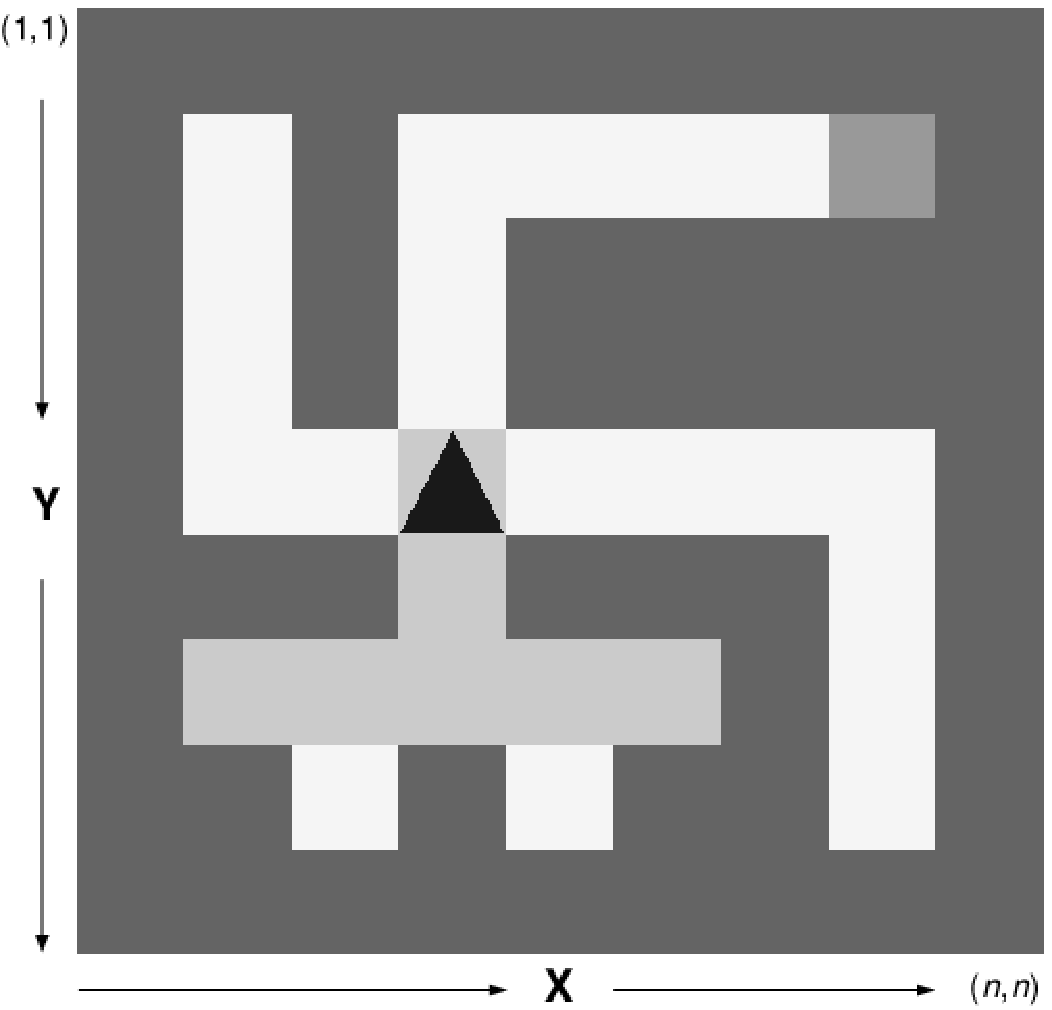
\includegraphics[width=3in]{pigs3.pdf}
\caption{The robot homing towards a target that is north-east would choose to 
go ahead (north) or right (east) as opposed to behind (south) or left (west). 
Note the relationship between the {\em x}- and {\em y}-coordinates of the robot 
and the target.
\label{northcontroller}}
\end{figure}    

\subsection{Exercise 3}

\noindent
The controller of the homing robot which we are going to 
build is based on a heading controller. \\

\noindent
Our new homing robot will choose a heading based on its current location 
and the location of the target. For instance,
if the robot is heading {\tt NORTH} and the target is to the north of it, as
in Figure~\ref{northcontroller}, then
it makes sense for the robot to select {\tt NORTH} in preference to 
{\tt SOUTH}. 
Based on this assumption, you will construct controller code to determine
whether
the target is to the {\em north}, {\em south}, {\em east} or {\em west} of 
the robot, and then 
build a heading controller that will guide 
the robot closer to the target.
Essentially what the robot is trying to do is `sense' the target and move 
towards it if at all possible. A scheme that seems inherently sensible, at 
least at the outset.

\subsubsection{Finding the target}

\noindent
It is possible to decide whether the target is to the north of the robot by 
examining the {\em y}-coordinate of the robot and the target\footnote{The 
coordinates begin (1,1) at the top left-hand corner of the maze and increase
to (n,n) at the bottom right-hand corner of the maze (the default maze is 15 by
15).}. If the robot's {\em y}-coordinate is greater than that of the target, 
then the target is north of the robot. Similarly, if the robot's 
{\em y}-coordinate is less than that of the target, then the target is to the 
south. If the {\em y}-coordinates of both the robot and target are the same, 
then you will find that both the robot and target are on the same latitude.\\

\noindent
$\diamondsuit$ Add a new method called {\tt isTargetNorth} to the file 
{\tt Broken.java}. The method should take one parameter (the robot 
itself\footnote{You will need this parameter if you are to check the 
{\em y}-coordinate of both the robot and target.}) and should return 
{\tt 1} if the target is north of the robot, {\tt -1} if the target 
is south of the robot and {\tt 0} otherwise.\\
\clearpage
\noindent
The method should look something like

\begin{verbatim}
   private byte isTargetNorth(IRobot robot) {
     byte result ...
     // returning 1 for `yes', -1 for `no' and 0 for `same latitude'
     ...
     return result;
   }
\end{verbatim}

\noindent
and should not be more than about five lines long.\\

\noindent
First sketch your solution on
paper, answering the following design questions as you go along: \\

\noindent
{\bf Design question 1:} Where in the
{\tt Broken.java} file should you locate this new method? \\

\noindent
{\bf Design question 2:} How can you determine the relative positions of 
the robot and the target? \\

\noindent
{\bf Design question 3:} What parts of the robot interface can help you 
in this calculation? \\

\noindent
Once your code compiles correctly, you should consider how to go about 
testing it. Is it possible to develop some exhaustive tests to cover all 
eventualities? You might want to look back to Section 3.3 of
{\em The Guide} to see what testing technique would me more appropriate.\\

\noindent
Consider adding some appropriate {\tt System.out.println} statements, 
and running the robot slowly to examine whether the output makes sense. 
You might find that moving the target and the robot will help you test 
more cases. Be prepared to talk about how you tested your solution and 
why you tested it in that way. \\

\noindent
$\diamondsuit$ Use your {\tt isTargetNorth} method as a basis for a second method
called {\tt isTargetEast}. This should return {\tt 1} if the target is to the 
east of the robot, {\tt -1} if the target is to the west of the target, and 
{\tt 0} otherwise.

\subsubsection{Sensing your environment}

\noindent
Currently the robot can sense its environment using the {\tt look()} function.
The function takes {\it relative} directions in order to operate correctly. The 
functions you have just written return the target's position in {\it absolute} directions 
and your controller will need to give the robot an {\it absolute} direction, so it makes
sense that you sense the environment using {\it absolute} directions. \\

\noindent
$\diamondsuit$ Write a method called {\tt lookHeading} that takes an {\it absolute} direction
and returns whether there is a {\tt WALL}, a {\tt PASSAGE} or a {\tt BEENBEFORE} square, much 
like the current {\tt look()} function. {\bf Hint:} You may need to pass the robot object to 
the function in addition to a heading.

\subsubsection{Building a heading controller}

\noindent
Using the methods that you have developed so far, it is 
possible to calculate where the target is relative to the current position of
the robot and to analyse the robots surroundings. 
As in Figure~\ref{northcontroller}, if we detect that the target
is to the north-east of the robot, it makes sense to direct it either 
north or east. That is, as long as there is not a wall in either (or both)
of these headings. \\

\noindent
$\diamondsuit$ Create a {\tt headingController} method that exhibits the following behaviour:

\begin{quote}
Given the state of the robot in the maze, the controller should {\bf return} a
heading that will head the robot towards the target if at all possible. 
This means that: ($i$) if it can select a heading that will move the robot
closer to the target then it should do so; ($ii$) it should not lead the 
robot into a wall; ($iii$) if the robot has the choice of more than one 
route, then it should randomly choose between them; ($iv$) if there
are no headings that will move the robot towards the target, pick randomly
between all available headings.
\end{quote}

\noindent
Before trying to write the software, you must have a clear understanding 
as to what this specification means exactly. \\

\noindent
{\bf Design question 1:} What should the robot controller do if travelling
{\tt NORTH} or {\tt EAST} will move the robot towards the target, and these 
passages are not blocked by walls? \\

\noindent
{\bf Design question 2:} What should the robot controller do if travelling
{\tt NORTH} or {\tt EAST} will move the robot towards the target, and there
is a wall to the north but not to the east? \\

\noindent
{\bf Design question 3:} What should the robot controller do if travelling
{\tt NORTH} or {\tt EAST} will move the robot towards the target, and there 
is a wall to the east of the robot but not to the north? \\

\noindent
Try to design your code on paper first. You might find it useful to create
a table of the scenarios that the robot might encounter and use this when 
designing your code.

\subsubsection{Testing your solution}

$\diamondsuit$ Now that the controller code is becoming more complex, it is 
important that we test it to see that it meets the desired functionality. \\

\noindent
To help with testing, we have constructed a {\em test harness} that you can
use to 
test your {\tt headingController}.  \\

\noindent
To access the test harness you need to first download it from the 
course web page; you will see that it is named {\tt ControlTest.class}
and it should be saved to the same directory as your source code. \\

\noindent
To call this test harness you need to add a couple of lines of code to 
your program. The first thing you should do is add a call to the test 
harness ({\tt ControlTest.test}) just before your robot sets its heading to the newly
chosen direction and advances, i.e.  

\begin{verbatim}
   ...
   heading = headingController(robot);
   ControlTest.test(heading, robot);
   robot.setHeading(heading);
   ...
\end{verbatim}

\noindent
This test-calling code will check each heading that your robot selects 
and compare it against a working solution. \\

\noindent
Next you need to add some code that will print the log of test results at 
the end of the robot's run. You should include the code

\begin{verbatim}
   public void reset() {
     ControlTest.printResults();
   }
\end{verbatim}

\noindent
to your class (outside the definition of the {\tt controlRobot} method,
 yet within the brackets of the whole class).\\

\noindent
These modifications will allow you to test the behaviour of your 
{\tt headingController} method. You should ensure that your robot passes 
these tests (indicated by a status report of {\bf ok}). Example test 
reports can be found on the course web page.\\

\noindent
Don't take this testing too lightly. If you were a customer buying the 
controller code then you would be pretty careful to check that it works,
particularly if you are paying good money for it.

\noindent
After thoroughly testing your solution, save it as {\tt Ex3.java}. 


\subsection{Final remarks}

\noindent
$\diamondsuit$
Can the homing robot always be expected to find the target? 
Carefully justify your answer. \\

\noindent
It is interesting that developing a smarter control algorithm does
not actually provide us with a better robot. The random robot
is preferable to the homing robot in the sense that it will eventually reach
the target, albeit after a very long wait. \\

\noindent
Also of interest is the fact that specifying and ordering a homing robot 
seemed sensible. It is quite possible that a customer, wanting a more  
sophisticated robot, would request such behaviour, unaware that the resulting 
robot would not reach the target in some cases.\\

\noindent
An answer to this sort of problem is to build a {\it prototype}. Software 
developers will often produce some small cheap code to model a potential 
solution to a coding problem. The code does not need to be shown to the 
customer, as in itself it is not important. What is important is the input and 
output behaviour that the code exhibits. A customer will be shown the 
prototype and asked to {\it inspect} the behaviour. It is at this point 
that the customer can say, `hang on, this was not what I thought it 
would do!'\\

\noindent
Prototypes are an excellent way of developing potentially expensive software.
They ensure that when a customer pays twenty million pounds for some code,
it turns out to be what they wanted.\\

\noindent
It is quite possible to write prototypes in the Java programming language,
but it is often argued that other languages are better suited to the task. For example, 
{\it functional} programming languages are favoured for the speed at which 
software can be developed and the size of the resulting code. They do not 
produce particularly fast code, but then again at the prototyping stage this 
probably does not matter. \\

\noindent
This is the end of the first coursework. Submit your work through the Tabula
submission system, making sure to include the following files:\\

\noindent
{\tt Ex1.java, Ex2.java, Ex3.java} \\

\noindent
This work will be tested on 
\deadlineone in Lab 001 of the Computer Science
building. If you have time, you might like to look through Chapters 6 and 
7 again just to make sure that you have fulfilled the requirements. Once 
you have done this you will be required to formally submit your work.
\clearpage
\section{Coursework 2 (Part 1): \\ Smarter Robot Controllers}

In the second coursework you are required to develop
sophisticated robot controllers which adopt a more systematic approach to
exploring a maze and that learn. In the first part of this coursework we will
initially build a controller that systematically searches a dense maze (one
that does not contain loops). In such mazes the
empty squares form a network (or tree) of corridors one square wide. 
There are additional exercises at the end of Part 1 whereby we extend
this controller
so that it is able to deal with loopy mazes\footnote{Mathematically this
means extending our robot from one that explores {\em trees} to one that
explores {\em graphs}.}.\\

\noindent
For the second part of the coursework you will be asked to
create a robot controller that learns from its previous runs. This means that
the more a robot explores (the same maze), the quicker it gets at finding the
target.\\

\noindent
To complete these exercises you will need to be familiar with the use of arrays in
Java. You will find plenty of examples dedicated to the use of arrays in the lecture
notes; you will also find good coverage of arrays in the recommended
course textbooks.\\

\noindent
The control programs which you will write will be more complicated
than those from the earlier chapters. As such, you will find that they are much
more manageable if you split them up by writing components as separate
methods. As a rough guide you should aim to keep each individual method
below 30 lines in length. Similarly, you will almost certainly find it
worth your while packaging useful bits of code from earlier questions (e.g.
choosing a random direction etc.) into methods for later re-use.\\

\noindent
In these exercises you are also required to develop your own Java class(es)
from scratch. This is an important part of code design and you will find that
you can reuse some of these classes in the solutions to the questions in
Chapter 9. It is important not to shy away from the inclusion of your own
classes. Apart from anything else, it will ensure that you gain a better
grade when your solutions are marked. \\

\noindent
This coursework, like the first, is split into two parts. You will find that
you are guided through the first part of the coursework but not the second.
The reason for this is that Part 2 is intended to be tricky and challenge the best students. 
Even if you do not complete
these every exercises, you may find that you pick up marks for partial 
solutions (or even non-working solutions), so it is worth having a go at these 
questions if you have time.\\

\noindent
All your solutions must
be complete by \deadlinetwo. You should remind
yourself of the rules for coursework by taking a quick look at the first page
of Chapter 6.


\subsection{Exercise 1}

$\diamondsuit$
An entirely new {\tt Explorer} robot controller is going to be built; this
should be done
in a file called {\tt Explorer.java}. This new controller should ensure
that the robot meets the following specification:

\begin{itemize}

\item
The robot should never reverse direction, except at dead ends.

\item
At corners it should turn left or right so as to avoid collisions.

\item
At junctions it should, if possible, turn so as to move into a square that
it has not previously been explored, choosing randomly if there are more than one.
If this is not possible it should randomly choose a direction that doesn't
cause a collision.

\item
Similar behaviour to junctions should be exhibited at crossroads:
the robot should select an unexplored exit if possible, selecting
randomly between the exits if more than one is possible. If there
are no unexplored exits then the robot should randomly choose a
direction that doesn't cause a collision.

\end{itemize}

\noindent As the specification suggests, there are four cases to
consider, the direction chosen if the robot is: at a dead end; travelling down
a corridor; at a junction; and at a crossroads.\\

\noindent
We can tell which of these cases we need to consider at any one time
by developing a method called {\tt nonwallExits}, running it and
observing the result. \\

\noindent
{\bf Design step 1:} Add a method {\tt nonwallExits} to your {\tt
Explorer.java} file which returns
the number of non-{\tt WALL} squares (exits) adjacent to the square currently
occupied by the robot. You will need to use the {\tt robot.look} method
and check all four directions. As a guide, your solution should not be more
than ten lines of Java code. \\

\noindent
You should check that you have not made any syntax errors by compiling your
solution. You will need to make sure that you have incorporated
the {\tt import} statement at the beginning of the file, you will also
need an {\tt Explorer} class which includes an empty {\tt controlRobot}
method as well as the new {\tt nonwallExits} method, e.g. \\

\begin{verbatim}
  import uk.ac...

  public class Explorer {
    public void controlRobot(IRobot robot) {}

    private int nonwallExits (IRobot robot) {  // Your new method
      ...
    }
  }
\end{verbatim}

\noindent
After some debugging you will find that the compiler no longer
complains. Of course you cannot run this
program yet as the controller code does not do anything. \\

\noindent
If the {\tt nonwallExits} method returns a result that is less
than two, then the robot is at a dead end; if the robot is
travelling down a corridor, then the number of non-wall exits
will be exactly two; if the number of non-wall exits is three
then the controller has detected that the robot is at a junction;
and finally, if the number of non-wall exits
is four then the robot is at a crossroads. See Figure~\ref{explorer} for details. \\

\noindent
A sensible way to proceed with the development of the explorer
robot is to design the method {\tt controlRobot} so that it
detects which of these four cases it is dealing with. If the robot
is travelling along a corridor, then the control method can pass
control to a subsidiary method which determines what to do in
this case. Likewise, the
dead-end, junction and crossroad cases can be developed in the same way. \\

\noindent
{\bf Design step 2:} Modify the {\tt controlRobot} method so that
it records the result of calling the {\tt nonwallExits} method. Store
the result in a variable called {\tt exits}. \\

\noindent 
{\bf Design step 3:} Now extend the  {\tt controlRobot}
method so that it passes control to four sensibly named subsidiary
methods depending on the value of the {\tt exits} variable.\\

\noindent
You will probably want these four subsidiary methods to return
direction values to your controller. Your controller therefore,
will need to introduce a variable {\tt direction} and assign the
result of calling the subsidiary method to that, e.g. \\

{\tt direction = deadEnd(robot);}\\

\noindent
The {\tt controlRobot} method will need to
execute the command {\tt robot.face(direction)} before it terminates. \\

\noindent
You can compile your changes to check for any syntax errors. You
will need to include empty definitions of your subsidiary methods
if the compilation is to succeed. The next task is to write the
four subsidiary methods. We will look at each of these in turn. \\

\begin{figure}[t]
\centering
\includegraphics[width=3in]{explorer.eps}
\caption{There is a clear relationship between the number of
non-wall exits and the situation which the {\tt Explorer} robot
finds itself in; this is demonstrated in the above figure.
\label{explorer}}
\end{figure}

\noindent {\bf Design step 4:} {\it Dead ends} -- What
should the robot do if it is at a dead end? Well, you are nearly
right. It should turn round and head back in the direction it
came from in all but one case -- when it is at the start. Write
the first of the four subsidiary methods to deal with the case
when the robot is at a dead end. This will not require too much
code as all you need to do is get the robot to find the one and
only non-wall route.\\

\noindent
{\bf Design step 5:} {\it Corridors} -- If the robot is travelling down a
corridor, or is at a corner, then control should be
passed to the corridor subsidiary method. This method will ensure that
when in a corridor the robot will not crash into walls (of course) and
that it will not reverse direction and go back on itself, since it only
does this at dead ends. Write this second subsidiary method; again it
should not be longer than about ten lines of code. \\

\noindent 
{\bf Design step 6:} {\it Junctions} -- At a junction
the robot controller should select a {\tt PASSAGE} exit if one
exists. This ensures that the robot explores new parts of the
maze in preference to exploring parts of the maze which it has
already visited. If there are no passage exits the robot should
choose randomly between all non-wall exits. \\

\noindent 
{\bf Design step 7:} {\it Crossroads} -- The final
subsidiary method is the control code for crossroads. This should
exhibit similar behaviour to that of the junction controlling
method: selecting an unexplored exit if possible, selecting
randomly between these unexplored exits if more than one is
possible and, if there are no unexplored exits, randomly
selecting a direction that doesn't cause a collision. \\

\noindent
You might find it useful to define an additional {\tt
passageExits} method. This will be similar to your {\tt
nonwallExits} method but instead it will return the number of
passage exits in relation to the robot position.\\

\noindent
Implementing the junction and crossroad control methods then
becomes simple. If there are one or more {\tt PASSAGE} exits then
the controller should choose one of the passages randomly; if
there are no {\tt PASSAGE} exits then the controller should choose
randomly between all non-wall exits. \\

\noindent
When you have completed the code you should compile it to remove all the
errors. When you have finished this you should have a new {\tt Explorer.class}
file which can be loaded into the robot-maze environment.
Test your robot controller carefully to ensure that it meets the specification.\\

%\noindent
%When you are satisfied that it works correctly, be sure to save
%the {\tt Explorer.java} file in {\tt Ex1.java} otherwise you will
%receive no marks for this exercise.

\subsubsection{Storing data}

$\diamondsuit$
You will notice that the explorer robot is very good when it comes to searching
areas of the maze which it has not been to before. However, when part of the
maze is thoroughly searched it is unfortunate that the robot goes into {\it random}
mode. It would be better if the robot were able to follow its path back to the
point at which it chose between one unexplored path or another. This
would enable the robot to backtrack to a previously encountered junction and
follow any previously unexplored exits. \\

\noindent
This is the behaviour of the robot controller which will be built in the
next two parts of this chapter. In order to do this,
the controller {\tt Explorer.java} will be modified so that, whenever
a junction is encountered which the robot has not previously encountered in its
current run, its location and the heading the robot arrived from are
recorded. This information will then be used in the implementation of a
{\it backtracking}~routine. \\

\noindent {\bf Design step 1:} You can easily detect whether a
junction or crossroads has already been visited during a robot run
by counting the number of adjacent {\tt BEENBEFORE} squares. If
there are more than one, the robot Explorer must have
visited the junction or crossroads at least once before. \\

\noindent Write a method called {\tt beenbeforeExits} that is
similar to the method {\tt passageExits} which you defined 
previously. This method will return the number of {\tt
BEENBEFORE} squares adjacent to the robot. \\

\noindent {\bf Design step 2:} The recording of junction and
crossroad information\footnote{From here on in the text I will
refer to junctions/crossroads simply as junctions. The smart
ones amongst you will have realised that there is in fact no
difference in the treatment of the two.} will be implemented in a
separate class which should be named {\tt RobotData}. This new
class can be included as part of the {\tt Explorer.java} file and
should contain local state
information for each junction the robot encounters. \\

\noindent When a junction is reached your robot should store the
{\it x}- and {\it y}-coordinates (to uniquely identify it) and the
{\it absolute} direction which the robot arrived from when it first encountered
this junction. This information can be stored in three arrays, i.e., 

\begin{verbatim}
 private static int maxJunctions = 10000; // Max number likely to occur
 private static int junctionCounter; // No. of junctions stored  
 private int[] juncX;            // X-coordinates of the junctions
 private int[] juncY;            // Y-coordinates of the junctions
 private int[] arrived;          // Heading the robot first arrived from
\end{verbatim}

\noindent An implementation which looked like this would be
quite adequate. However, you might decide that an array of {\tt
JunctionRecorder} objects or
something similar would be a better implementation (and indeed it would).\\

\noindent
The coordinates and arrived-from direction for the {\em i}-th
freshly unencountered junction will be stored in the {\em i}-th
elements of the arrays. You can do this by using an integer
variable ({\tt junctionCounter}, say) to count the number of
junctions for which information has been recorded.\\

\noindent
On the first pass of a new run {\tt junctionCounter} should be
set to 0. This can be done by observing the {\tt robot.getRuns()}
method which allows the control program to detect when it is
computing the first run through a maze (see Section 4.2.9). This
value alone is not enough as it will remain 0 throughout the
robot's first run through the maze. What you need to do is
include a counter which counts the number of times the controller
code is polled. A combination of these values will allow you to
detect the first move in a first run through a
new maze. \\

\noindent
The code for this might look something like: \\

\begin{verbatim}
  public class Explorer {
    private int pollRun = 0;     // Incremented after each pass
    private RobotData robotData; // Data store for junctions
    ...

    public void controlRobot(IRobot robot) {
      ...
      // On the first move of the first run of a new maze
      if ((robot.getRuns() == 0) && (pollRun == 0))
         robotData = new RobotData(); //reset the data store
      ...
      pollRun++; // Increment pollRun so that the data is not
                 // reset each time the robot moves
    }
  ...
\end{verbatim}

\noindent where the constructor code for {\tt RobotData} does
something sensible -- such as setting {\tt junctionCounter} to
zero, for example. \\

\noindent
Complete and insert this code into the {\tt Explorer.java} file. \\

\noindent
This is a tricky part of the Explorer code as you are having to
manage the introduction of your new {\tt RobotData} class as well
as interfacing with the maze-environment itself. In order to pull
this off you need to add the method

\begin{verbatim}
   public void reset() { 
      robotData.resetJunctionCounter(); 
   }
\end{verbatim}

\noindent to the {\tt Explorer} class in which you are developing
your controller code, and then add to your {\tt RobotData} class
the method \\

\begin{verbatim}
   public void resetJunctionCounter() {
      junctionCounter = 0; 
   }
\end{verbatim}

\noindent What this does is ensure that when you press the {\bf
Reset} button in the maze-environment your {\tt junctionCounter}
variable will be reset\footnote{You must follow these
instructions otherwise you will get into 
trouble in the next exercise.}. \\

\noindent {\bf Design step 3:} Now modify the {\tt controlRobot}
method so that each time the robot arrives at a previously
unencountered junction the coordinates and the direction the
robot arrived from are stored in the {\tt junctionCounter}
elements of each
array. Remember to increase the {\tt junctionCounter} by 1. \\

\noindent
A nice way to carry out this recording of junction information is to extend
the {\tt RobotData} class so that
it includes a {\tt recordJunction} method. This method might take three
parameters: the {\em x}-coordinate of the junction (which you can access
by making a call to {\tt robot.getLocation().x}); the {\em y}-coordinate of
the junction (which you can access by making a call to
{\tt robot.getLocation().y});
and the robot heading (which you can access by calling
{\tt robot.getHeading()}).\\

\noindent
{\bf Design step 4:}
When you have completed these modifications, test that the information
recorded is
correct by printing it out on the screen (using a {\tt printJunction()} method)
and comparing it with the simulation display. \\

\noindent
If you are in any doubt as to what the result of this exercise is
then consider the following scenario: In Figure~\ref{helpful} we
see that the robot has passed through three junctions. In this
case one would expect the robot to record (and print using
the {\tt printJunction()} method) the following information:

\begin{figure}[t]
\centering
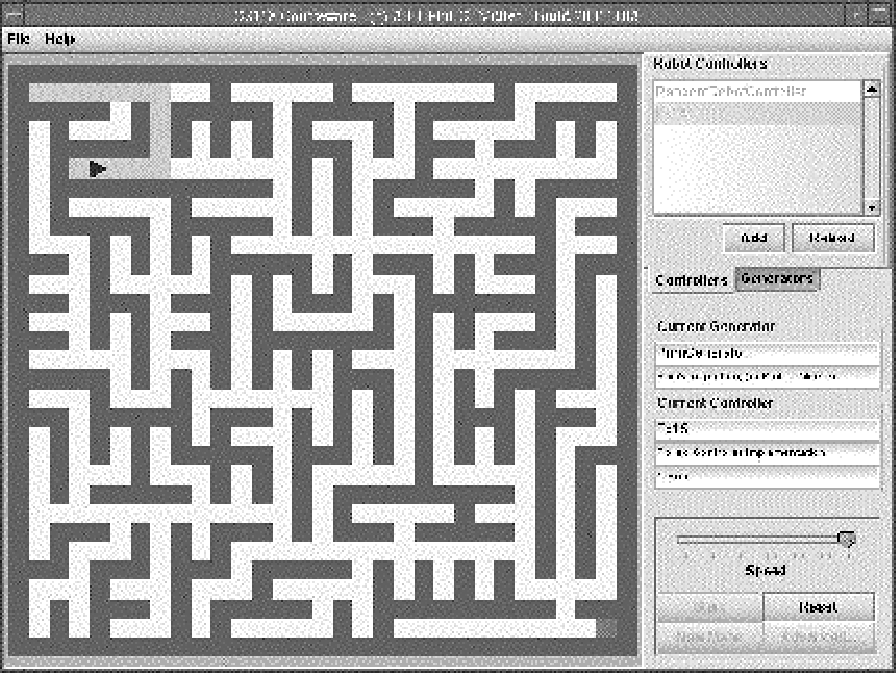
\includegraphics[width=4.5in]{helpful.pdf}
\caption{The robot has passed through three junctions. The information
which is stored in your new {\tt RobotData} class includes the x- and
y-coordinates of these junctions as well as the heading of the robot 
as it arrived at these junctions.
\label{helpful}}
\end{figure}

\begin{verbatim}
    Junction 1 (x=5,y=1) heading EAST
    Junction 2 (x=7,y=1) heading EAST
    Junction 3 (x=7,y=5) heading SOUTH
\end{verbatim}

\noindent
In order to verify that the output of your program is correct in
relation to the movement of the robot, you will have to run your
robot very slowly. Reset your robot every now and then and trace
through the route of the robot and the output you get from {\tt
printJunction()}, just to make sure that the information which you
record is correct.

%\noindent
%Save your answer to this exercise as {\tt Ex20.java}.
%Remember, no file, no marks.


\subsubsection{Using stored data}

$\diamondsuit$
Modify the {\bf Explorer} robot so that it uses the information it records to
perform a systematic search for the target. The specification for the new
robot is as follows:

\begin{itemize}

\item
Initially the robot will {\em explore}.

\item
When the robot is {\em explore}-ing it behaves like the original
{\tt Explorer} robot except that when it reaches a dead end or a junction
that it has already encountered in the same run, it should reverse direction
and {\em backtrack}.

\item
If the robot encounters a junction with unexplored exits while
{\em backtrack}-ing it should choose one of these exits randomly
and {\em explore} down it.

\item
If the robot encounters a junction with no unexplored exits while
{\em backtrack}-ing it should {\em backtrack} in the direction from which
it came when it first reached the junction. This behaviour is termed
`backtracking through' a junction.

\end{itemize}

\noindent
All this may sound complicated but it is not. What the robot controller is
really doing here is switching between two states, the {\em exploring}
state and the {\em backtracking} state. This switch can be implemented as
a state variable of the {\tt Explorer} class,

\begin{verbatim}
  private int explorerMode;  // 1 = explore, 0 = backtrack
\end{verbatim}

\noindent
for example. \\

\noindent
{\bf Design step 1:}
Add the {\tt explorerMode} variable to your code and set it in your
control code so that when the robot begins a new run the mode is
appropriately initialised\footnote{The robot should start off in explorer mode.
You can ensure that this is the case by adding an appropriate line of code just
after your call to {\tt new RobotData();}. To ensure that you get the same
effect when the {\bf Reset} button is pressed, you should also add this line
of code to the {\tt reset()} method which you introduced in the previous
exercise.}. \\

\noindent
We now need to implement two controllers,
{\tt exploreControl} and
{\tt backtrackControl}. The robot will be able to
switch between these states depending on the
situation. \\

\noindent
{\bf Design step 2:}
The method {\tt exploreControl} is pretty much the same code as you
used previously. You should define a new method called
{\tt exploreControl} in your {\tt Explorer} class.
When you have done this, cut the explorer code out of {\tt controlRobot}
and paste it into {\tt exploreControl}. You will find that the
{\tt controlRobot} method then contains just the basic
control code which detects if it is a new run etc. and of course, a call
to the new {\tt exploreControl} method.\\

\noindent
To complete the {\tt exploreControl} method you also need to add
the code which sets the {\tt explorerMode} switch to zero when you reach
a dead end. \\

\noindent
{\bf Design step 3:}
The {\tt backtrackControl} method will require a call to a
{\tt searchJunction} method (which should also be defined as part of your
{\tt RobotData} class) which is used to search the {\tt RobotData}
for a junction which has already been encountered. This will return the
direction that the robot was travelling when it originally arrived at the
junction. \\

\noindent
Write the method {\tt searchJunction} which, when given the {\it x}- and
{\it y}-coordinates of the robot, will return the robot's heading when it
first encountered this particular junction.  What will this method
return if it is called when the robot is at a junction which it has not
previously encountered? \\

\noindent
{\bf Design step 4:} Your backtracking control method can now be
written. Start by introducing a new method {\tt backtrackControl},
below your {\tt exploreControl} method, in the {\tt Explorer} class.
Design your backtrack
control method so that it calculates the number of non-wall exits
in relation to the robot's position -- this is a similar framework to
the {\tt exploreControl} function.\\

\noindent
If the number of non-wall exits is greater than two, then the
robot is at a junction or crossroad. The backtracking control method
then needs to detect if there are any {\tt passageExits} at this junction:
if there are, then the robot must switch back into explorer mode
and then proceed down one of these unexplored paths (choosing
randomly between them if there are more than one); if there are
no passage exits then the robot must exit the junction the
opposite way to which it FIRST entered the junction. You can use
the {\tt searchJunction} method to determine the initial heading
of the robot when it first entered the junction -- the controller
should calculate the reverse of this and head the robot in that
direction\footnote{See Section 5.2.4.}.\\

\noindent
If the number of non-wall exits is two or less, then the backtracking
method should use the existing methods which select a direction at a
corridor and select a direction at a dead end respectively. \\

\noindent
{\bf Design step 5:} There is one further design step which you need to make
and that is to consider what the controller should do when the robot is
at the very first square. \\

\noindent
If you have any doubts as to what all this means then talk to your
seminar tutor. Time will be set aside in the seminars to discuss these set of
problems. \\

\noindent Save your answer to this exercise as {\tt Ex1.java}. No
file; no marks.

\subsubsection{Worst case analysis}

$\diamondsuit$
Will the robot {\bf Explorer} always find the target using this strategy? Can you place
a limit on the length of time (or maximum number of steps) it will take {\bf Explorer} to find the target?
Explain your answers.


\subsection{Exercise 2}

In a `real life' situation it may be highly desirable to minimise the amount
of data storage required by the control program. \\

\noindent
$\diamondsuit$ Re-implement your robot controller so that the systematic search strategy of
the {\bf Explorer} robot does not require the \emph{location} of
each junction to be recorded. \\

\noindent
Save your solution to {\tt Ex2.java}.


\subsection{Depth-first search in path finding}

Throughout this chapter you have been working on the solution to a
well-documented {\it search problem}. These sorts of problems are ubiquitous,
cropping up everywhere in Artificial Intelligence and in other areas of
Computer Science.\\

\noindent
Imagine taking our maze and picking it up from the robot's start position.
You can lift the maze up so that it hangs like a mobile; it will look
like an inverted tree (see Figure~\ref{mobile}). You will notice that each path through
the maze becomes a branch in the tree, terminating at a leaf when a
dead end is reached. The target will appear on one of the branches in the
tree.\\

\begin{figure}
\centering
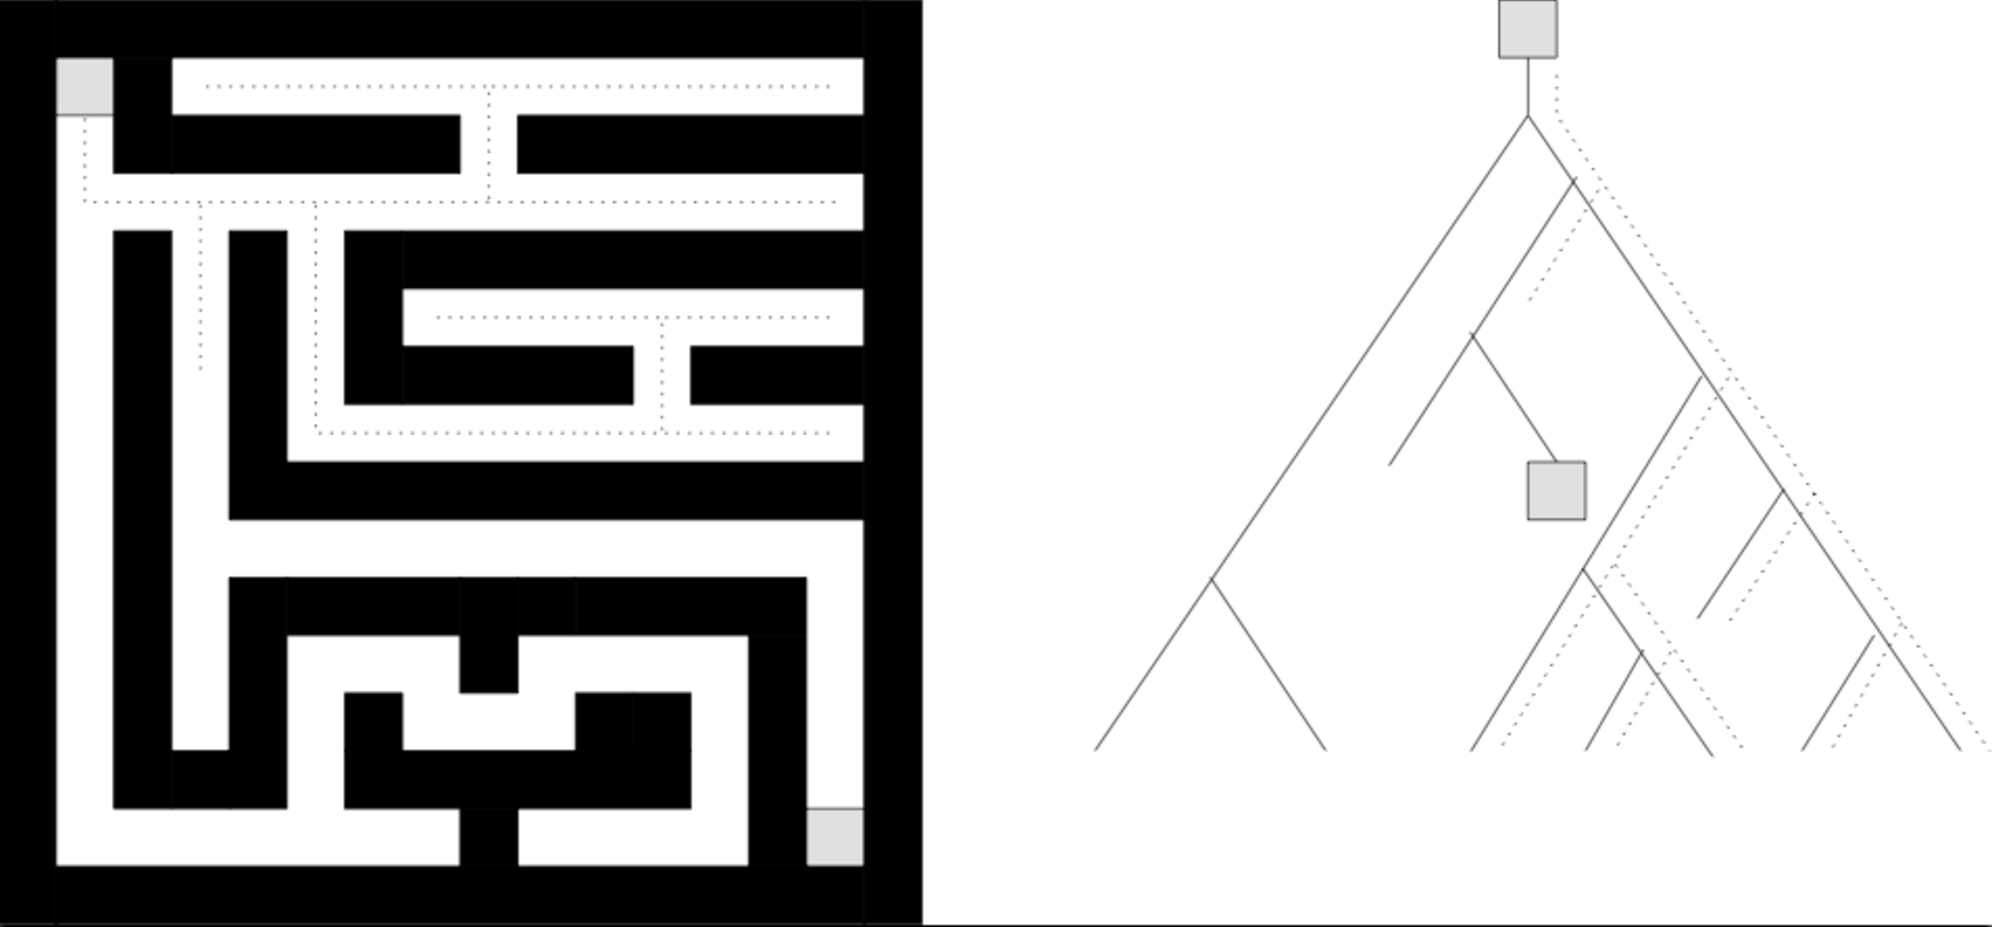
\includegraphics[width=4in]{mobile.pdf}
\caption{Representing the maze as a search tree \label{mobile}}
\end{figure}

\noindent
Consider what happens when the explorer robot searches the maze. First it
will choose one path of the maze. The robot will thoroughly search the part
of the maze which this path leads to; any unexplored exits will be
searched until, if the target is not detected, the robot backtracks to the
junction at which the initial choice was made.\\

\noindent
This procedure is analogous to searching one part of the maze-tree. Given
that one initial path is as likely to be as good as any other, searching
the tree requires picking an alternative at every node in the tree and
working forward from that alternative. Other alternatives at the same
level are ignored as long as there is a hope of reaching the
target using the original choice. This search strategy is known as
a {\it depth-first search}.\\

\noindent
The search proceeds to the bottom of the tree if the target is not found;
it then backs up to the nearest ancestor node with an unexplored alternative.
If this path does not work out then the procedure will move still further
back up the tree seeking another viable decision point to move forward from.
This process continues until the target is reached or all possible paths in
the tree are exhausted. \\

\noindent
There are many other search techniques which are used to solve this and
similar problems in Computer Science. Some of these search techniques will
be more efficient, others will be more suited to finding the {\it shortest
path}. Special-case procedures also exist which are appropriate when
facing an adversary. These procedures use {\it game trees} and are common
in computer programs that play board games such as chess for example.

\subsection{Exercise 3}

\subsubsection{Single loops}

Currently our {\bf Explorer} robot uses a depth-first search. This is all very 
well as long as our maze is non-loopy -- as soon as a loop is introduced the
exploring algorithm breaks\footnote{You can test this out for yourself.}.\\
 
\noindent
$\diamondsuit$ Modify your {\bf Explorer} robot so that it is able to navigate mazes with 
single loops. Some of you may find it easier to work from your Exercise 1 answer,
others may find it easier to extend from Exercise 2. \\

\subsubsection{Multiple loops}

$\diamondsuit$
Extend your answer so that your robot can navigate
mazes with multiple loops. \\

\noindent
Save your solution to {\tt Ex3.java}. \\

\noindent
Solving loopy mazes has been the subject of much research\footnote{From
longer ago than you might think -- from the ancient Minoans in Crete in
about 2000~BC, to our very own upper-class and bored Royalty, with nothing better
to do than frolic around in daft clothes and in houses large enough
to host a maze in their outside privy.}
and as you might expect, someone has already contemplated the problem of
navigating around a maze with multiple loops. Indeed a nice solution to
this problem was originally published in {\em Recreations Mathematique}
(Volume 1, 1882) by M. Tr\'{e}maux. 

\subsection{Summing up}

You have now reached the end of the first set of exercises of Coursework 2.
Getting this far in the exercises will probably be enough to ensure that you
get a pass grade for the practical component of the
Programming for Computer Scientists course (providing your
code works, has comments, looks nice etc.)
Before you go off and celebrate, you must ensure that you 
submit a copy of the files {\tt Ex1.java}, {\tt Ex2.java}, and {\tt Ex3.java}.  \\

\noindent
Make sure that you change the class name at the top of each file from 
{\tt Explorer} to {\tt Ex*} such that they compile correctly. Then submit your
solutions through Tabula.

\clearpage
\section{Coursework 2 (Part 2): \\
         The Grand Finale}

The exercises in this chapter are designed to test the very best of you. 
Although it should be said that it is 
possible to get a good grade in the practical component of the CS118 
course without having done the exercises in this chapter; 
this means that if you do 
not get a chance to finish this part then you should not panic. You may 
however find the exercises interesting and decide that you have time to 
attempt some or all of the questions provided. Even if you do not complete 
the exercises, you might get some marks for trying. So even if your robot 
is a bit wonky, you may still gain credit for a part solution. \\

\noindent
In this second part of Coursework 2 you are required to design, build and 
test a {\em learning robot}. You will receive much less step-by-step 
guidance and as a result I expect to see lots of exciting and innovative 
solutions. Your solutions will be marked on design, programming style and 
of course correctness\footnote{If your program works then you can be 
assured of at least 60\% of the marks, if you have a smart design then 
you will bank a further 20\%, and if you have programmed like a coding god 
then you can expect the remaining 20\% of the marks.}.\\

\noindent
The programs which you will write for this section are probably the most 
interesting in this course. You will produce some very clever robot 
controllers as answers to the questions. It can also be very satisfying to 
watch the more advanced robots in action. \\

\noindent
As a consequence of the work being more difficult, you will receive extra 
credit for any work you do from this chapter. It is very difficult to quantify
exactly what this means in terms of {\it your} marks, as other factors such as 
programming style, reusability, etc. will play a part. However, you might 
like to think of these exercises as constituting the difference between an 
{\em A} grade and a {\em B} grade in your coursework (depending on 
where the grade boundaries are drawn). \\

\noindent
This year there will also be a prize for the person who develops the 
best solution. You could win this by going beyond the specification, or
perhaps you could produce the shortest solution to the grand finale\footnote{The current
record for shortest solution is 5 lines of code, including all of the Java filler! Though a submission
of 30 lines or below would be very impressive for first year students.}. Previous
winners have also turned the maze environment into a game, and created interesting 
graphical displays to show the maze-tree as it was being explored.

\subsection{The {\it Grand Finale}}

You receive a call from NASA. They have seen your robot in action and plan 
to use some of your code in their next mission\footnote{Heaven forbid.}. 
However, while it is clear that your robot searches in a very sophisticated 
way, NASA point out that it does not learn from its mistakes\footnote{Unlike
NASA, of course.}. What they would like is a robot that learns. \\

\noindent
$\diamondsuit$ The aim of this last part is to build a {\bf learning robot} that can use 
information gathered during previous runs through a maze to find a target at 
increasing speed. \\

\noindent
The plan is to build on your previous solution. The robot will
search the maze (in its {\bf Explorer}-like way) the {\em first time} 
the robot is run through a maze but, 
the {\em second time}\footnote{or more} the robot is run, it will use its 
virtual map (its memory if you like) to find the target more quickly.
What you would expect the robot to do the second time round is exclude the 
routes through the maze which went nowhere and instead select those which
it knows will take it towards the target. \\

\begin{figure}[t]
\centering
\includegraphics[width=4.5in]{finale1.eps}
\caption{A trace of the {\bf GrandFinale} robot the first run through the 
maze.
\label{finale1}}
\end{figure}    

\begin{figure}[t]
\centering
\includegraphics[width=4.5in]{finale2.eps}
\caption{A trace of the {\bf GrandFinale} robot the second time it 
runs through the maze.
\label{finale2}}
\end{figure}    

\noindent
An example of this behaviour is demonstrated in Figures~\ref{finale1} 
and~\ref{finale2}. In Figure~\ref{finale1} we see the trace of the robot the 
first time it is run through a fairly extensive maze. As you would expect it 
is fairly thorough about the areas which it explores, 
finally however it reaches the target.\\

\noindent
When the robot is run again, shown in Figure~\ref{finale2}, the robot can 
use the information which it stored about the maze during the first run to 
direct its search for the target. As you see it needs far less exploration 
the second time round. The aim of the second part of Coursework 2 is to 
model this behaviour. \\

\noindent
There is more than one way of doing this and in order to provide you with 
some (modest) assistance I shall describe two approaches which you might 
like to take. I do not mind which of these you go for, if any.

\subsection{Route A}

$\diamondsuit$
Modify {\bf Explorer} so that it records the junctions (if any) 
that each known junction's exit(s) lead to. Test that your program stores the
correct information by temporarily modifying it to print the information on
the screen and comparing the results with the layout of small test mazes.
The information gathered should be retained between runs in the same maze.\\

\begin{figure}
\centering
\includegraphics[width=3.8in]{junc_info.eps}
\caption{Storing more junction information.\label{7.1}}
\end{figure}

\noindent
You may wish to experiment with the use of complex data structures
or arrays of arrays
to record this information in a conveniently accessible form. Figure~\ref{7.1}
shows the sort of data structure which you will need and the extra information
which you are likely to store. Note that as well as storing the 
direction from which the robot entered a junction, the controller also stores 
the junction 
which taking a {\tt LEFT}, {\tt RIGHT}, {\tt BEHIND} or {\tt FORWARD} path 
would lead to. \\

\noindent
In the figure you will see that the array index at which the information relating
to a particular junction is stored, provides a very
convenient means of identifying that junction. Since these identifying
integers will be positive (or zero), exits which have yet to be explored can
be represented as a negative number. Remember that a method is
provided which tells you whether you are computing the first run
in a maze, and using this you can detect whether the maze has changed since 
the previous runs. \\

\noindent
The second task is to
design, build and test a method which uses the information collected by
the controller to compute a route between the start and end of the maze. \\

\noindent
My advice here is to think first and implement second! Consider how you might
represent and compute such a route. Give yourself time to think. Go away from
the computer, with pencil and paper (or coffee, or beer, whatever...) to 
design a good scheme. Then try to implement and test your ideas. If inspiration
fails to strike even after thinking hard, your seminar tutor will be able to
offer a hint or two. There are quite a number of possible methods which you could
use, and each can be implemented as a computer program in many different
ways. So, don't panic if your solution sounds completely different to that 
offered by the seminar tutor -- the chances are that you are both right. \\

\noindent
Save your working implementation to this exercise in the file 
{\tt GrandFinale.java}.

\subsection{Route B}

$\diamondsuit$
There is a solution to this problem which many perceive as simpler to that 
presented in Route A. This route is based on your answer to Exercise 2 and 
so you might like to remind yourself what that was about.\\

\noindent
It is possible to store the arrived-from direction and not the x- and 
y-coordinates of the robot and still build a learning robot. What you need to 
do in this case is treat the arrived-from directions as a {\em stack} of 
values. \\

\noindent
The analogy which is often introduced when describing stacks in Computer 
Science is a pile of dinner plates. If you imagine this pile, then plates can
only be introduced at the top of the pile (if you want to avoid any lifting)
and similarly taking a plate (in this lazy way) means taking one from 
the top as opposed to anywhere else in the pile. This method of putting 
things on and taking things off is described as {\em last in first out}, and 
Computer Scientists use the terms {\em push}ing items onto the stack and 
{\em pop}ing them off. \\

\noindent
You can use a stack to record the arrived-from directions of the robot. Each
time the robot arrives at a junction the arrived-from direction should 
be pushed onto the stack; when the robot is backtracking the arrived-from 
directions should be popped off the top of the stack. \\

\noindent
If you use this approach you will find that by the time the robot reaches
the target the stack will contain a route to the target. The trick is to 
then use this stack the next time round to direct the robot straight to the 
target.\\

\noindent
Save your working implementation to this exercise in the file 
{\tt GrandFinale.java}.

\subsection{Submitting your coursework}

The files which should be submitted for the second coursework are {\tt Ex1.java},
{\tt Ex2.java}, {\tt Ex3.java} and also {\tt GrandFinale.java}.\\

\noindent
In order to make the marking of your work easier, you should make sure that the
class names correspond to the file names -- that is, file {\tt Ex2.java} 
contains the definition \\

{\tt public class Ex2} \\

\noindent
and similarly for the other files. \\

\noindent
Submit your working using Tabula, as before. The marking of this coursework will take place on
\deadlinetwo. Be there or be square\footnote{In fact, be there 
or get no marks.}.

\subsection{Epilogue}

This coursework has touched on a number of different areas of Computer 
Science. You have learnt something about {\em specifications} and {\em 
refinement}, you have learnt something about {\em programming} and 
{\em software testing}. You will have also touched on {\em data structures}
and {\em algorithms}, and also {\em AI}. \\

\noindent
There is much to learn in the remainder of your degree course but this 
should give you an idea as to how all these areas fit together and how 
important each is in its own right. \\

\noindent
Programming is a complicated business and you are not going to have mastered 
it in ten weeks. It is a bit like learning to drive -- you have probably 
crashed a few times already, or at least come off the road -- and you 
will get better the more you do. By the summer many of you will be taking 
up well paid summer jobs fixing peoples' Java code. This may sound hard to 
believe right now, but each year it is the same; the only thing that 
changes is that the wages go up!


%\input{overview.tex}
%\input{books.tex}
%\input{timeline.tex}
%\input{coursework.tex}
%\input{exam.tex}
%\input{guidance.tex}

%\clearpage 
%\section{Lecture notes}

%\subsection{Lecture 10: \lectureTenTitle}
%\label{sec:lecture-10}

%\input{lecture10.tex}



%\clearpage
%\section{Exercises}

%\input{lectures/lecture1.tex}
%\input{lectures/lecture2.tex}
%\input{labs/lab1.tex}

%\input{lectures/lecture3.tex}
%\input{lectures/lecture4.tex}
%\input{labs/lab2.tex} \newpage

%\input{lectures/lecture5.tex}
%\input{lectures/lecture6.tex}
%\input{labs/lab3.tex}

%\input{lectures/lecture7.tex}
%\input{lectures/lecture8.tex}
%\input{labs/lab4.tex}

%\input{lectures/lecture9.tex}
%\input{lectures/lecture10.tex}
%\input{labs/lab5.tex} \newpage

%\input{lectures/lecture11.tex}
%\input{lectures/lecture12.tex}
%\input{labs/lab6.tex} \newpage

%\input{lectures/lecture13.tex}
%\input{lectures/lecture14.tex}
%\input{labs/lab7.tex} \newpage

%\input{lectures/lecture15.tex}
%\input{lectures/lecture16.tex}
%\input{labs/lab8.tex} \newpage

%\input{lectures/lecture17.tex}
%\input{lectures/lecture18.tex}
%\input{labs/lab9.tex}

%\input{lectures/lecture19.tex}

%\clearpage
%\section{Solutions and how to find them}

%This section contains model answers for selected exercises along with descriptions of how I obtained them.

%\input{labs/sol3.tex}

\end{document}